%%%%%%%%%%%%%%%%%%%%%%%%%%%%%%%%%%%%%%%%%%%%%%%%%%%%%%%%%%





%
% Vzor pro sazbu kvalifikační práce

%
% Západočeská univerzita v Plzni


% Fakulta aplikovaných věd
% Katedra informatiky a výpoetní techniky
%
% Petr Lobaz, lobaz@kiv.zc.cz, 2016/03/14
%
%%
%%%%%%%%%%%%%%%%%%%%%%%%%%%%%%%%%%%%%%%%%%%%%%%%%%%%%%

% Možné jazyky práce: czech, english
                                                                                                                                                                                                                                                                        % Možné typy práce: BP (bakalářská), DP (diplomová)
\documentclass[czech,BP]{thesiskiv}


% Definujte údaje pro vstupní strany



%
% Jméno a příjmení; kvůli textu prohlášení určete, 



% zda jde o mužské, nebo ženské jméno.
\author{Miroslav Havlíček}
\declarationmale

%alternativa: 
%\declarationfemale





% Název práce

\title{Analýza a vizualizace dat z ubytovacích portálů}





% 
% Texty abstraktů (anglicky, česky)
%

\abstracttexten{The text of the abstract (in English). It contains the English translation of the thesis title and a short description of the thesis.}

\abstracttextcz{Cílem této práce je výběr nástroje k analýze a vizualizaci dat z ubytovacích portálů, zodpovězení zadaných otázek pomocí dat z ubytovacích portalů a vytvoření interaktivních webových stránek k zobrazení vizualizací. Data jsem zpracovával pomocí nástroje Kibana a výsledné vizualizace jsou zobrazeny na webových stránkách. Stránky vznikly kombinací technologií HTML, JavaScript a PHP. Výsledkem jsou odpovědi na deset otázek, které jsou podpořeny vizualizacemi. Hlavním přínosem je možnost srovnání dvou hotelů, což je umožněné filtry a různými vizualizacemi.
}
% Na titulní stranu a do textu prohlášení se automaticky vkládá 
% aktuální rok, resp. datum. Můžete jezměnit:

%\titlepageyear{2016}
%\declarationdate{1. března 2016}
% Ve zvláštních případech je možné ovlivnit i ostatní texty:%
%\university{Západočeská univerzita v Plzni} 
%\faculty{Fakulta aplikovaných věd}
%\department{Katedra informatiky avýpočetní techniky}








%\subject{Projekt 5}
%\titlepagetown{Plzeň}
%\declarationtown{Plzni}



















%%%%%%%%%%%%%%%%%%%%%%%%%%%%%%%%%%%%%%%%%%%%%%%%%%%%%%%%%%
%







% DODATEČNÉ BALÍČKY PRO SAZBU
% Jejich užívání či neužívání záleží na libovůli autora 


\usepackage{listings}
\usepackage{amsmath}
\usepackage{siunitx}






                 
% práce
%
%%%%%%%%%%%%%%%%%%%%%%%%%%%%%%%%%%%%%%%%%%%%%%%%%%%%%%%%%%

% Zařadit literaturu do obsahu

\usepackage[nottoc,notlot,notlof]{tocbibind}

% Umožňuje vkládání obrázků
\usepackage[pdftex]{graphicx}
\usepackage{tikz}
\usepackage{pdfpages}


\def\todo#1{\bgroup \textcolor{red}{TODO: (#1)}\egroup}








% Odkazy v PDF jsou aktivní; navíc se automaticky vkládá
% balíček 'url', který umožňuje např. dělení slov
% uvnitř URL
\usepackage[pdftex]{hyperref}
\hypersetup{colorlinks=true,
  unicode=true,
  linkcolor=black,
  citecolor=black,
  urlcolor=black,
  bookmarksopen=true}
% Při používání citačního stylu csplainnatkiv
% (odvozen z csplainnat, http://repo.or.cz/w/csplainnat.git)
% lze snadno modifikovat vzhled citací v textu
\usepackage[numbers,sort&compress]{natbib}

%%%%%%%%%%%%%%%%%%%%%%%%%%%%%%%%%%%%%%%%%%%%%%%%%%%%%%%%%%
%
% VLASTNÍ TEXT PRÁCE
%
%%%%%%%%%%%%%%%%%%%%%%%%%%%%%%%%%%%%%%%%%%%%%%%%%%%%%%%%%%
\begin{document}
%
\maketitle
\tableofcontents
\chapter{Úvod}
Hlavním úkolem této bakalářské práce je zanalyzovat a vizualizovat data z ubytovacích portálů. Tato data jsou uložena v databázi Elasticsearch, která byla zvolena, protože se jedná o nestrukturovaná data. Data představují recenze z hotelů v okolí Dubaje, která byla získána z ubytovacích portálů. Tyto recenze byly zpracovány skupinou NLP, která působí na Fakultě aplikovaných věd Západočeské univerzity. Úkolem této práce tudíž není připravit data a uložit je do databáze, ale využít tato data k zodpovězení otázek pro Zayedovu univerzitu z Dubaje.


Databáze Elasticsearch byla zvolena díky možnosti ukládání velkých dat, pro které je typická jejich rozsáhlost a běžně dostupné databázové nástroje nejsou schopny tyto data zpracovat v rozumném čase, především kvůli velkému množství nestrukturovaných vazeb.\cite{BigData} První částí této bakalářské práce je prozkoumání různých nástrojů sloužících k vizualizaci dat, které jsou dostupné na trhu. Tyto nástroje jsou nejčastěji součásti aplikací Bussiness Intelligence, což jsou aplikace sloužící k analýze, reportování a vizualizaci velkého množství dat, které podniky sbírají a následně je využívají jako podporu pro strategické rozhodování. 

Důležitým kritériem pro výběr nástrojů k analýze dat je podpora ukládání a zpracování nestrukturovaných dat. Nestrukturovaná data jsou běžně reprezentována fotografiemi, zvukovými nahrávkami, daty ze senzorů, ale také například  souvislým textem, což je náš případ. S výběrem databáze Elasticsearch souvisí i výběr vizualizačního nástroje, kterým je nástroj Kibana. Ten slouží k vizualizaci dat z nástroje Elasticsearch skrze webové uživatelské rozhraní.


Dalším úkolem bakalářské práce je tvorba webových stránek, které budou zobrazovat vybrané vizualizace, jenž v rámci práce vzniknou. Hlavní funkcionalitou by mělo být snazší porovnání vybraných hotelů podle zadaných kritérií, než je tomu u nástroje Kibana, který není pro běžné uživatele snadno ovladatelný.


Kapitola \ref{Nástroje_1} je zaměřena na porovnání dostupných nástrojů a jejich detailnější představení. Kapitola \ref{Funkce_nástroje} pojednává o možnostech vizualizace tohoto nástroje a jeho dalších rozšíření. Další kapitola obsahuje odpovědi na vybrané otázky a jejich vizualizace. Kapitola \ref{chap:WEB} je tvořena popisem webových stránek a využitých technologií. Poslední částí bakalářské práce je zhodnocení práce, za kterou následuje slovníček pojmů, ve kterém je možné dohledat vysvětlení odborných termínů a zkratek.


\chapter{Nástroje k analýze a vizualizaci dat }
\label{Nástroje_1}
První kapitola práce je zaměřena na nástroje, pomocí kterých je možné analyzovat a vizualizovat semi-strukturovaná popřípadě nestrukturovaná data. Na trhu je mnoho nástrojů určených pro zpracování firemních dat a většinou jsou součástí komplexnějšího řešení ve formě BI nástroje. BI je zkratka pro Business Intelligence, což je rámocvý termín pro škálu aplikací, které slouží k analýze nestrukturovaných dat organizace.\cite{BI}

\section{InetSoft Style Intelligence}
Jedná se o produkt firmy InetSoft Technology Corporation, která  se zaměřuje na vývoj BI aplikací. Společnost nabízí aplikace určené k tvorbě podnikových reportů a k vizualizaci vlastních firemních dat. Tyto aplikace jsou založené na webových technologiích a například aplikace Vizualize Free a Style Scope Free Edition jsou zdarma. Při vývoji se především používá XML, což je obecný značkovací jazyk pro uchování a přenos dat, SOAP, což je protokol pro přenos XML zpráv přes síť, Java a JavaScript\cite{InetTechnology}. Hlavně díky použití programovacího jazyka Java, který je dnes celosvětovou jedničkou mezi programovacími jazyky \cite{JavaStandings} jsou aplikace snadno integrovatelné s jinými aplikacemi, které jsou dostupné jako open-source. Open-source aplikace jsou distribuovány s licencí, která dovoluje upravovat původní zdrojový kód aplikace a následně již upravenou verzi aplikace dále distribuovat jako open-source.

\subsection{Přehled}
InetSoft Style Intelligence je velmi silný nástroj, který umožňuje zpracovat a kombinovat data z různých zdrojů. Systém je nabízen jako cloud aplikace nebo jako řešení na míru. Cloudové aplikace jsou v dnešní době oblíbeným řešením, protože nekladou nároky na hardware uživatele a navíc jsou všechny operace prováděny na serverech poskytovatele těchto aplikací. Výhodou cloudu je, že uživatelé platí jen za výpočetní kapacitu, kterou skutečně využijí a jedná se tak o finančně výhodnější řešení, než-li hosting, kdy se platí za celý server, i když není zcela využitý. Řešením na míru je například produkt InetSoft Style, který je nasazen přímo na server subjektu a společnost InetSoft garantuje minimální zatížení serveru.

\subsection{Technologie}
\subsubsection{Kolekce dat}
Základem je technologie Data Block\texttrademark, která zprostředkovává shromažďování dat z různých zdrojů. Data z databáze získává tento nástroj přímo z originálních úložišť pomocí předem připravených materializovaných pohledů. Tyto pohledy představují databázové objekty, ve kterých je uložen výsledek nějakého dotazu, takže je přístup k něme rychlejší než provádění nového dotazu.

\subsubsection{Zpracování dat}
Po kolekci a přípravě dat je možné z dat tvořit různé vizualizace, které slouží k lepšímu pochopení dostupných dat. InetSoft Style poskytuje uživatelům dashboardy, které se v pravidelně aktualizují podle dat, které jsou k dispozici, a ze kterých je dashboard tvořen. Dashboardy mohou být tvořeny jednoduchými grafy, složitějšími multidimenzionálními grafy, které jsou vhodné pro porovnání hodnot, a nebo například geografickými mapami. InetSoft Style zároveň obsahuje sadu předpřipravených dashboardů například pro oblast zdravotnictví, vzdělávání nebo podpory prodeje a nákupu. 


\subsection{Kompatabilita}
Firma tvrdí, že její produkt je schopný převzít data z téměř jakéhokoliv zdroje, což zvládá díky jejich data mashup engine. Zákazník tedy může použít jak strukturovaná tak semi-strukturovaná nebo dokonce nestrukturovaná data. InetSoft Style Intelligence podporuje export do běžných formátů, díky čemuž jsou data a grafy využitelné například v aplikacích balíčku MS Office. Jelikož se jedná o službu založenou na webové technologii, tak je dostupná na všech hlavních prohlížečích na běžných systémech jako jsou Windows, Unix, Linux, Mac OS X, HP-Unix, Solaris a další.\cite{InetKompatilbilita}

\subsection{Hodnocení a ceník}
Hlavní výhodou tohoto produktu je uživatelsky přívětivé prostředí, kde uživatelé tvoří vizualizace svých dat. To je zapříčiněno především přehledností webové stránky, ze které se nástroj ovládá. Jednotlivá tlačítka zlehčují ovladatelnost systému a také systém drag and drop, který umožňuje používat nástroj bez nutnosti znalosti dotazovacího jazyka. Velkým pozitivem je i možnost ovládat nástroje přes mobilní telefon, ale podle mého názoru je to vhodné jen k zobrazování již vytvořených analýz a dashboardů. Dalším pozitivem je i možnost nahlédnout přímo do původních dat pouhým kliknutím na libovolný prvek vizualizace. Výhodou je taktéž to, že produkt není určen primárně pro technicky vzdělané uživatele, ale je určen pro běžné uživatele bez nutnosti podpory IT oddělení. Balíček služeb je dostupný již od 2 800 dolarů.\cite{InetCenik} Pozitivní je, že produkty Vizualize Free a Style Scope Edition jsou zdarma na neurčitou dobu. Oba produkty jsou založeny na cloud technologii a akceptují pouze strukturovaná data.



%--------------------------------------SPLUNK------------------------------------------------------------
\section{Splunk Enterprice}
Software byl vytvořen firmou Splunk Inc., která se zaměřuje na vývoj podpůrného softwaru pro vyhledávání, analyzování a monitoring strojových dat skrze webové rozhraní.\cite{Splunk_a_kompatibilita} Splunk Enterprise patří mezi základní produkty této firmy, ale ta dále nabízí cloudovou verzi Enterprise pod názvem Splunk Cloud\texttrademark a Splunk Light, což je nástroj na monitoring logů pro menší IT subjekty. Základní verze těchto produktů je možno rozšířit o další nadstavby a vytvořit tak komplexní řešení na míru každého zákazníka. Mezi nadstavby patří produkty Splunk Enterprise Security, který se zaměřuje na kolekci a analýzu dat získaných ze zabezpečovacích technologií, Splunk IT Service Intelligence, což je nástroj na sledování funkčnosti IT systémů (sleduje podezřelé aktivity systému, výkon systému a předem definované kritické částí systému), a Splunk User Behaviour Analytics, který používá strojové učení k detekci potencionálních hrozeb a kyberútoků. Právě díky nástrojům vhodným ke zlepšení kyberbezpečnosti spolupracuje firma s americkou vládou skrze zprostředkovatelskou firmu.\cite{Splunk_security}

\subsection{Přehled}
Produkt Splunk Enterprise je vhodný pro sběr, analýzu a úpravu strojových dat ve velkém množství (tzv. Big Data). Tato data mohou být generována různými interními systémy uživatele ve formě serverových logů, aplikačních logů, dat o výrobě, logů ze sociálních sítí a podobně. Software je určen primárně pro zpracování semi-strukturovaných a nestrukturovaných dat z non-SQL databází.

\subsection{Technologie}
\subsubsection{Kolekce dat}
Velkou výhodou tohoto řešení je nezávislost na formě vstupních dat, protože ty jsou zpracována a zaindexována do formy, kterou produkty od firmy Splunk vyžadují, zcela automaticky. Nedochází však k normalizaci dat, ale data jsou uchovávána v raw podobě, na které odkazují metadata v souborech s indexy. Raw data jsou nezpracovaná data, která nemají přiřazenou informační hodnotu.

\subsubsection{Vyhledávání}
Vyhledávání je zprostředkováno vlastním query jazykem, který se jmenuje Search Processing Language neboli SPL\texttrademark. Jazyk je velmi rozsáhlý a obsahuje více než 140 příkazů. Výsledky z vyhledávání jsou interpretovány do vhodných interaktivních grafů, které jsou zvoleny přímo aplikací na základě množství a formy dat. Vyhledává se buďto pomocí SPL\texttrademark nebo přes velké množství filtrů a případně kombinovaně. \cite{Operational_intelligence}

\subsubsection{Zpracování dat}
Jelikož je vytvořen soubor s indexy, tak Splunk Enterprise zvládá korelaci a analýzu z různých zdrojů najednou, což značně urychluje práci analytikům. K tvorbě modelů a k predikci anomálií v chování systému používá produkt strojové učení. Modely lze vytvářet přímo skrze webový prohlížeč pomocí speciálních příkazů jazyka SPL\texttrademark. Jako základ strojového učení jsou použity knihovny programovacího jazyka Python. \cite{MachineLearning}


Data se vizualizují pomocí různých uživatelsky přizpůsobitelných grafů, které se následně skládají do interaktivních dashboardů, které lze posléze exportovat ve formě HTML. Výhodou je, že lze nastavit uživatelská práva jednotlivým dashboardům, přiřadit jim ovládací prvky a následně je sdílet s ostatními kolegy skrze společný pracovní prostor.


\subsection{Kompatibilita}
Splunk je zaměřen především na zpracování big dat, ale je možné ho připojit i na relační databáze, nebo ho propojit s tabulkovým procesorem Microsoft Excel či produktem Tableau, který je podrobně popsán v sekci 1.3. Splunk lze rozšiřovat vlastními aplikacemi, nebo lze využít databázi Splunkbase, kde jsou již vytvořené aplikace a rozšíření, které umožňují lepší integraci a vizualizaci. K aplikaci je také možné se připojit přes mobilní zařízení a kontrolovat tak chod sledovaného systému. Splunk je možné provozovat pod operačními systémy Linux, Windows 7 a novější a pod operačním systémem Mac OS X. \cite{Splunk_a_kompatibilita}

\subsection{Hodnocení a ceník}
 Ke každému produktu jsou k dispozici zkušební verze, které jsou omezeny jak časově, tak množstvím přenesených dat. Od množství přenesených dat za den se odvíjí i cena produktu, ale je k dispozici produkt Splunk Free, který je určen pro jednotlivce a má omezené funkce monitoringu a strojového učení. Velkou výhodu spatřuji v existenci vlastní komunity, která zprostředkovává možnost přímo se zeptat uživatelů na přínosy, popřípadě je to místo, kde hledat pomoc při problémech se softwarem od společnosti Splunk Inc.
 
 
 %--------------------------------------TABLEAU------------------------------------------------------------
 \section{Tableau Desktop}
 Jedná se o produkt americké softwarové společnosti Tableau Software, jenž se zaměřuje na vývoj softwaru vhodného pro vizualizaci dat a na nástroje business intelligence. Firmu založili lidé, kteří se účastnili výzkumu v oblasti vizualizace dat. Konkrétně se jednalo o projekt Polaris, který byl veden katedrou počítačových věd Standfordské univerzity.\cite{TableauHistory} Mezi hlavní produkty firmy patří kromě Tableau Desktop taktéž Tableau Server, který je určený především pro spolupráci napříč organizací, Tableau Online, což je cloudová verze produktu Tableau Server, Tableau Public, který je určen pro jednotlivce na nekomerční užití a proto je zdarma, a Tableau Reader, který je taktéž volně dostupný a slouží k prohlížení a manipulaci vizualizací vytvořených některým produktem Tableau. Produkty od firmy Tableau jsou dnes především využívané datovými žurnalisty, kteří oceňují jejich snadnou ovladatelnost.
 
 \subsection{Přehled}
 Tableau Desktop je nástroj k analýze a vizualizaci vlastních dat a také nástroj business intelligence. Produkt je nabízen ve verzi Personal, která je určena osobnímu použití a vstupní data musejí být strukturovaná, a ve verzi Professional, která zvládá i nestrukturovaná Big Data. Výhodné je spojení s produktem Tableau Server, aby bylo možné vytvořené dashboardy a ostatní vizualizace sdílet s kolegy. Předností produktu Tableau Desktop je uživatelská přívětivost, protože k jeho běžnému používání nejsou nutné žádné pokročilé technologické znalosti, ale stačí používat systém tvorby vizualizací drag and drop. 
 
 \subsection{Technologie}
 \subsubsection{Kolekce a příprava dat}
 Aby Tableau Desktop umožňovala používání dat z více zdrojů, je nutné jejich předzpracování, na což využívá vlastní nástroj, který sám hledá vztahy mezi jednotlivými zdroji dat a uživatele tak příliš nezatěžuje. Zdroje dat rozlišuje do dvou hlavních skupin, a to na soubory (například z MS Excel, MS Access, textových souborů, logů a podobně) a na databázové servery, na které je možné produkt Tableau Desktop přímo napojit. Data se pak mohou přenášet buďto přímým spojením, nebo technologií in-memory, kdy se přenáší jen virtuální obraz dat a Tableau tak pracuje rychleji bez nutnosti odesílání velkého množství dotazů serveru.


 Z projektu Polaris vznikl dotazovací jazyk VizQL\texttrademark. Jedná se o vizuální query jazyk, který převádí jednotlivé drag and drop příkazy na dotazy.\cite{VizQL} Výhodou je lepší ovladatelnost pro méně technicky zdatné uživatele, protože se nemusí orientovat v dotazovacích jazycích a mohou přímo vidět výsledky vizualizací pomocí systému drag and drop.

 \subsubsection{Zpracování dat}
 Data jsou rozdělena na dvě kategorie, na dimenzionální (jména, regiony) a kvantitativní data (množství, prodeje, zisk …). Výhodou jsou filtry dat, které jsou aplikovatelné na více různých zdrojů dat najednou. U Tableau je ceněno seskupování dat, což je funkce, která automaticky seskupí data, která mají společné vlastnosti (například geografickou polohu, symptomy nemocí) a následně lze tyto data v grafu zvýraznit, či je přesunout do nově vzniklého grafu.\cite{TableauDimensions}


 Tableau nabízí mnoho analytických nástrojů a umožňuje provádět výpočty nad daty při tvorbě dashboardů. U dashboardu je po zveřejnění možnost ho hodnotit, popřípadě okomentovat, čehož následně využívají již zmíněné analytické nástroje, které tvoří žebříček oblíbených, případně trendy dashboardů. Obrovská výhoda Tableau je správa dashboardů. Kromě nastavování uživatelských práv lze i sledovat vývoj dashboardu pomocí interního verzovacího systému.\cite{TableauVersion}
  
 \subsection{Kompatibilita}
 Tableau Desktop nabízí možnost využít základní aplikaci pro modifikovatelný přístup k datům a vizualizacím a jelikož je napsána v JavaScriptu je možné ji dále rozšiřovat dle vlastních potřeb. Pomocí této aplikace lze vizualizace exportovat do jiných programů především z rodiny MS Office. Aplikace je založena na webových technologiích, takže je kompatibilní s běžnými distribucemi Windows 7 a vyšší a s Mac OS X 10.10 a novější. Verzi Personal je možné propojit se zdroji dat typu MS Access popřípadě přímo s textovými soubory ve formátu CSV popřípadě JSON. CSV soubory jsou určeny pro výměnu tabulkových dat, která obsahují data vzájemně od sebe oddělená odělovačem (například čárkou, středníkem, tabulátorem atd.). JSON \uv{neboli JavaScript Object Notation je formát souborů určený k výměně dat.}\cite{JSON} Je snadno čitelný i zapisovatelný člověkem a zároveň lze soubory ve formátu JSON snadno generovat i zpracovávat strojově. Tableau Desktop verze Professional je již propojitelná s většinou databázových systémů, které se dnes používají (např. Oracle Databases, PostgresSQL, Cloudera Hadoop Hive and Impala, Cisco Information Server).\cite{TableauSources}
 
 \subsection{Hodnocení a ceník}
 Cena se pohybuje od 999\$ za osobní verzi, až po 1999\$ za profesionální edici Tableau Desktop.\cite{TableauPricing} Zajímavostí je, že firma nezapomněla na své kořeny ze Stanfordské univerzity a je tak pro všechny studenty a vyučující k dispozici zdarma bez omezení. Verze Tableau Public, která je zdarma pro širokou veřejnost, má podobné vizualizační nástroje jako placené verze, ale podporuje zpracování pouze již strukturovaných dat. Stejně jako u produktu Splunk Enterprise má Tableau vlastní komunitu, která je podporována přímo firmou Tableau a kam přispívají jak jednotliví zaměstnanci, tak i zákazníci. K dispozici je taktéž mobilní aplikace, která je primárně určená pro prohlížení vytvořených dashboardů. 
 
 
 %--------------------------------------SISENSE------------------------------------------------------------
 \section{Sisense}
  Tento software je produktem stejnojmenné firmy, která se zaměřuje na nástroje buisiness intelligence. Jejich řešení jsou komplexní a obsahují jak nástroje na sběr dat, tak nástroje na jejich vizualizaci. Společnost je uváděna jako lídr oblasti poskytovatelů buisiness intelligence nástrojů a její produkty se v očích odborné veřejnosti tak i v očích uživatelů jeví jako velmi spolehlivé.\cite{SisenseStandings}
 
 \subsection{Přehled}

 Sisense je koncový BI nástroj, který byl vyvinut pro uživatele, kteří nemají téměř žádné zkušenosti s BI nástroji a nemusejí být technicky zdatní. Aplikace nabízí nástroje pro správu, text mining a pro interaktivní analýzu dat, která jsou uložena v databázi ElastiCube, což je podpůrný produkt Sisense. Výhodou Sisense je velmi snadná ovladatelnost pomocí systému drag and drop, bez nutnosti znalosti query jazyka.

 \subsection{Technologie}
 \subsubsection{Kolekce a příprava dat}
  Sisense nevyžaduje časově náročnou fázi předzpracování dat, tak jako ostatní BI nástroje na trhu. Data z různých zdrojů jsou sjednocena a importována do jednotného úložiště, což usnadňuje práci s daty a nevyžaduje nákup speciálních programů na přípravu dat, popřípadě spouštění skriptů nad daty. Databáze ElastiCube je sloupcově orientovaná a je tvořena mnoha poli, kde každá hodnota v polích má odpovídající logickou hodnotu v jiném poli a tím je databáze propojena. Proto je vhodné používat tento typ uložení při velkém množství dat, nebo pokud jsou data z různých zdrojů.


  Výhodou je také zpracování jednotlivých dotazů, které nejsou na rozdíl od běžných technologií zpracovány jako celek, ale jsou rozděleny do bloků, které se následně vyhodnocují. To je výhodné časově, protože při jednotném zpracování dotazů musí CPU při každé změně v dotazu opětovně vyhodnotit celý dotaz zatímco při blokovém musí zpracovat jen tu část dotazu, která byla změněna.\cite{ElasticCube}


  Rychlost, za kterou je produkt velmi ceněn, je dána způsobem zpracování dat, který je na rozdíl od ostatních produktů na trhu zajištěn technologií in-chip. Tato technologie je v databázových systémech jedinečná a jejím základem je maximalizace využití paměti, kterou poskytují jednotlivé CPU, protože přístup do této paměti je výrazně rychlejší, než přístup do paměti RAM, která je využívána technologií in-memory.

 \subsubsection{Zpracování dat}
 Vizualizace je umožněna širokou paletou grafů a geografických map, které lze skládat do interaktivních real-time dashboardů. Tyto dashboardy se následně mohou sdílet napříč organizací a sledovat jeho vývoj a případně upravit uživatelská práva. Každý dashboard obsahuje ovládací panely s filtry a lze zde přímo upravit znění dotazů a přizpůsobit tak vizualizace dle aktuálních potřeb. Aplikace již obsahuje některé dashboardy předpřipravené, což je určeno především pro nezkušené uživatele.\cite{SisenseVizualize}
 		
 \subsection{Kompatibilita}
  Nabízí předpřipravené nástroje na import dat z Excelu, Google Adwords, Salseforce, CRM reports, Splunk bez nutnosti složitého importu dat, což je opět určeno především pro netechnické uživatele, kteří dokáží pomocí systému drag and drop jak importovat a zpracovat data, tak je následně vizualizovat a popřípadě exportovat například do formátů CSV, PDF, Excel a podobně. \uv{PDF je formát používaný k prezentaci a spolehlivé výměně dokumentů, který je nezávislý na softwaru, hardwaru i operačním systému.}\cite{PDF} Aplikace Sisense je založena na webových technologiích a je tak kompatibilní s běžnými operačními systémy jako jsou Windows, Android, Mac OS X. Splunk nabízí možnost obohatit produkt o řadu předpřipravených rozšíření, nebo je možné  přímo vyvíjet rozšíření v JavaScriptu, kdy je ovšem doporučeno toto rozšíření konzultovat s komunitou.\cite{SisenseAdd-ons}

 \subsection{Hodnocení a ceník}
 Cena softwaru se odvíjí od objemu společnosti a od velikosti zpracovávaných dat, ale je k dispozici až na konkrétní dotaz. K dispozici je i demo verze, která již obsahuje data a je tak možné si vyzkoušet funkcionalitu systému před jeho zakoupením. Výhodou je napojení systému na mobilní telefony. Co se týče zpracování strojových dat, sám výrobce doporučuje propojení Sisense s produkty od firmy Splunk. Stejně jako Tableau a Splunk, podporuje Sisense vlastní komunitu.\cite{SisenseAndSplunk}
 
 
 %--------------------------------------Kibana------------------------------------------------------------
 
 \section{Kibana}
 Kibana je open source nástroj na vizualizaci dat od firmy Elastic a byla vytvořena jako plugin do fulltextového vyhledávače Elasticsearch, který vychází z Apache Lucene. Elasticsearch je NoSQL bezschémová databáze, což znamená, že není nutné definovat předem přesnou strukturu databáze, ale databáze sama nastaví schéma podle dat, která obsahuje. NoSQL jsou databáze nové generace vhodné pro zpracování velkého množství dat.\cite{NoSQL} Přesto se u Elasticsearch doporučuje zvolení alespoň základního schématu, což může usnadnit následné analýzy nad daty.\cite{SchemaElastic} Oba nástroje jsou součástí produktu Elastic Stack, který je jediným produktem firmy Elastic a je dostupný jako open source. Dále jsou k  dispozici rozšířené funkce, které je ovšem již nutné zakoupit. Elastic Stack se skládá z Elasticsearch, Kibana
 , Logstash a Beats.
 
 \subsection{Přehled}
 Kibana byla původně vytvořena jen jako plugin k Elasticsearch, ale nyní je z ní plnohodnotná součást celku Elastic Stack a je hojně využívána především pro monitorování logů ze serverů. Kibana umožňuje spojit data z databáze do komplexních grafických prvků, ze kterých je snazší datům přiřadit význam. Díky rychlosti databáze Elasticsearch a jejím možnostem fulltextového vyhledávání můžeme aplikaci Kibana nazývat real-time nástrojem, pokud jsou tedy správně zaindexována data, které obsahuje databáze. Problémem může být pro některé uživatele ovladatelnost, která není tak jednoduchá jako například u Tableau i přes přítomnost systému drag and drop. Na druhou stranu je ceněné rychlé vyhledávání buďto skrze všechna data, nebo skrze data, která si pomocí dotazu vybereme.

 \subsection{Technologie}
 \subsubsection{Kolekce a příprava dat}
 Jelikož je Kibana součástí produktu Elastic Stack, který obsahuje i Elasticsearch, nemusí se řešit ukládání dat, ale stačí definovat indexování, které odpovídá indexům v Elasticsearch. Indexy lze přidat i za běhu aplikace v záložce \uv{Settings}. Při vypracování používám Kibana ve verzi 5.1.1, která obsahuje indexy \uv{hospitality} a \uv{new\_index}.

 \subsubsection{Prohlížení dat}
 Data lze přímo prohlížet skrze webovou aplikaci na záložce \uv{Discover}, kde jsou zobrazena všechna data přidaná za časový úsek, který lze měnit v pravém horním rohu stránky. Data jsou zobrazena v tabulce, kde jsou rozepsány jednotlivé skupiny dat, nebo je možné zobrazit soubor ve formátu JSON, který je přímo uložený v databázi. Jednotlivé záznamy lze řadit podle data přidání a je možné změnit rozložení tabulky vybráním specifických skupin dat ze seznamu, který je po levé straně webové stránky.

 \subsubsection{Zpracování dat}
 Záložka \uv{Vizualize} slouží ke grafickému vyjádření dat z databáze Elasticsearch například ve formě plošných grafů, spojnicových grafů, kruhových grafů nebo například jako geografickou oblast. Jednotlivé vizualizace lze ukládat do komplexnějších dashboardů, které lze upravovat na záložce \uv{Dashboards}. Dashboardy lze tvořit z vizualizací, které vznikly na základě různých indexů, což nebylo v předchozích verzích možné a hlavně jedna vizualizace může být využita ve více dashboardech, protože existuje jako samostatný objekt.


 Filtry lze použít přímo v jednotlivých objektech, nebo nad celými daty. Filtrování lze provádět pomocí speciálních query dotazů zadávaných do vyhledávacího pole nad vizualizacemi, daty či dashboardy. Dále je možné filtry využít již při vytváření vizualizace a poté je jen pomocí ovládacích prvků v horní části vizualizace spravovat, nebo využít filtrů, které nabízí Kibana na základě struktury dat, která byla použita při vizualizaci.\cite{KibanaQueries}
 
 \subsection{Kompatibilita}
	Kibana je napsána v JavaScriptu a využívá architektury klient-server. Jelikož patří do Elastic Stack, který je distribuovaným systémem, tak je snadno integrovatelná s jinými nástroji. Například od verze 5 lze přímo skrze Kibanu vkládat do Elasticsearch data ve formátu CSV, což umožňuje integraci s nástrojem Microsoft Excel. Problémová je kompatibilita se staršími verzemi Kibany, kdy je naprosto nutné upgradovat nejprve Elasticsearch, protože každá verze má jinou strukturu clusterů, což je kolekce serverů, která shromažďuje data a poskytuje indexování a vyhledávání přes jednotlivé servery.\cite{KibanaClusters}
 
 \subsection{Verze 5}
 V říjnu roku 2016 vyšla verze 5.0, kdy Kibana doznala především grafických změn, které na její funkčnost nemají velký význam. Ke změnám funkcionalit lze řadit nezobrazování histogramu záznamů u dat, která neobsahují časovou značku, což na rozdíl od předchozí verze šetří čas při zobrazování logů. Velmi podstatnou změnou je odstranění linku nad jednotlivými záznamy v databázi, které mohly způsobovat bezpečnostní riziko, jelikož odkaz vracel reálný JSON soubor uložený v Elasticsearch skrze prohlížeč a volání GET. Toto se změnilo a nyní je k dispozici pouze náhled, který neodkazuje na JSON a je tak bezpečnější ho sdílet. Novinkou je také generování krátkých URL odkazujících na vizualizace či dashboardy, což je více uživatelsky přívětivé, než předchozí dlouhé URL adresy. Novinkami jsou i nové nabídky na hlavní liště, která byla přesunuta na levou stranu a je skryta, když není používána, což zvětšuje prostor k zobrazení vizualizací. Navíc přibyly nástroje Timelion a Console, což dříve byly jen pluginy. Timelion je nástroj, který umožňuje sledovat změny v čase v jednotlivých datech. Console je nástroj, který usnadňuje psaní query dotazů. Dotazy lze skládat do jednoho souboru, dělit je podle indexů a nástroj má dokonce funkci našeptávače, který ještě více usnadňuje psaní dotazů. Co se týče možností rozšiřování kódu, doznala verze 5 také vylepšení, protože jednotlivé položky hlavního menu byly rozděleny do samostatných pluginů, které se dají lépe upravovat. Další novinkou je možnost upravovat názvy os u jednotlivých vizualizací, jelikož se v nabídce objevil nový parametr s názvem \uv{Custom Label}. U filtrů, které lze připnout nad vizualizace taktéž přibyla možnost přímé úpravy query dotazu a lze tak ovlivnit chování daného filtru. \cite{Kibana5intro}

 
\section{Srovnání produktů}
Tabulka \ref{Srovnání_produktů} slouží ke srovnání jednotlivých produktů podle 14 kritérií, které jsem zvolil na základě průzkumu trhu s nástroji k analýze a vizualizaci dat.
Legenda pro tabulku \ref{Srovnání_produktů}:
\begin{itemize}
	\item[] \tikz\draw[black,fill=black] (0,0) circle (.5ex); : Pouze v kombinaci s produktem Tableau Server.
	\item[] \tikz\draw[black, thick] (0,0) circle (.5ex); : Pouze v kombinaci s produktem X-Pack.
	\item[] \tikz\draw[red,fill=red] (0,0) circle (.5ex); : Verze Personal od 999\$ ročně a verze Professional od 1999\$ ročně.
	\item[] + : Produkt splňuje kritérium.
	\item[] - : Produkt nesplňuje kritérium.
	\item[] * : Doživotní licence omezená přenosem 5GB za den. Cena za GB.
	\item[] ** : Cena za roční licenci.
	\item[] F : Produkt je zdarma.
	\item[] X : Cena je individuální dle dodávaných řešení.
\end{itemize}

\begin{table}[htbp]
	\centering

	\begin{tabular}{|l|c|c|c|c|c|c|c|c|}
		\hline
		\multicolumn{1}{|c|}{\begin{tabular}[c]{@{}c@{}}Kritérium/\\Produkt\end{tabular}} & 
		\begin{tabular}[c]{@{}c@{}}{\rotatebox[origin=c]{90}{ InetSoft Style }}\end{tabular} &
		\begin{tabular}[c]{@{}c@{}}\rotatebox[origin=c]{90}{ Splunk Enterprise }\end{tabular} &
		\begin{tabular}[c]{@{}c@{}}{\rotatebox[origin=c]{90}{ Splunk Free }}\end{tabular} &
		\begin{tabular}[c]{@{}c@{}}{\rotatebox[origin=c]{90}{ Tableau Desktop }}\end{tabular} &
		\begin{tabular}[c]{@{}c@{}}{\rotatebox[origin=c]{90}{ Tableau Public }}\end{tabular} &
		\begin{tabular}[c]{@{}c@{}}{\rotatebox[origin=c]{90}{ Tableau Reader }}\end{tabular}
		& \begin{tabular}[c]{@{}c@{}}{\rotatebox[origin=c]{90}{ Sisense }}\end{tabular} &
		\begin{tabular}[c]{@{}c@{}}{\rotatebox[origin=c]{90}{ Kibana }}\end{tabular} \\ \hline
		Dashboardy                                                                         & +                                                        & +                                                           & +                                                     & +                                                         & +                                                        & -                                                        & +       & +      \\ \hline
		\begin{tabular}[c]{@{}l@{}}Kompatibilita\\ s Elasticsearch\end{tabular}            & -                                                        & -                                                           & -                                                     & -                                                         & -                                                        & -                                                        & -       & +      \\ \hline
		\begin{tabular}[c]{@{}l@{}}Export do\\ MS Office\end{tabular}                      & +                                                        & +                                                           & +                                                     & +                                                         & +                                                        & -                                                        & +       & +      \\ \hline
		\begin{tabular}[c]{@{}l@{}}Kompatibilita\\ s OS\end{tabular}                       & +                                                        & +                                                           & +                                                     & +                                                         & +                                                        & +                                                        & +       & +      \\ \hline
		\begin{tabular}[c]{@{}l@{}}Vlastní\\ komunita\end{tabular}                         & -                                                        & +                                                           & +                                                     & +                                                         & +                                                        & +                                                        & +       & +      \\ \hline
		\begin{tabular}[c]{@{}l@{}}Podpora \\ nestrukturo-\\ vaných\\ dat\end{tabular}     & +                                                        & +                                                           & +                                                     & +                                                         & -                                                        & -                                                        & +       & +      \\ \hline
		\begin{tabular}[c]{@{}l@{}}Podpora\\ NoSQL\\ databází\end{tabular}                 & +                                                        & +                                                           & +                                                     & +                                                         & +                                                        & -                                                        & +       & +      \\ \hline
		\begin{tabular}[c]{@{}l@{}}Sdílení\\ vizualizací\end{tabular}                      & +                                                        & -                                                           & -                                                     &  \tikz\draw[black,fill=black] (0,0) circle (.5ex);                                                         & +                                                        & -                                                        & +       & +      \\ \hline
		\begin{tabular}[c]{@{}l@{}}Strojové učení\\ na detekci\\ anomálií\end{tabular}     & -                                                        & +                                                           & +                                                     & -                                                         & -                                                        & -                                                        & +       & \tikz\draw[black, thick] (0,0) circle (.5ex);      \\ \hline
		\begin{tabular}[c]{@{}l@{}}SW na kolekci\\ dat\end{tabular}                        & +                                                        & +                                                           & +                                                     & +                                                         & -                                                        & -                                                        & +       & +      \\ \hline
		\begin{tabular}[c]{@{}l@{}}Uživatelská\\ práva\end{tabular}                        & +                                                        & +                                                           & -                                                     & +                                                         & -                                                        & -                                                        & +       & -      \\ \hline
		\begin{tabular}[c]{@{}l@{}}Webová aplikace\end{tabular}                        & +                                                        & -                                                           & -                                                     & -                                                         & -                                                        & -                                                        & +       & +      \\ \hline
		\begin{tabular}[c]{@{}l@{}}SW  na \\ zpracování \\ dat\end{tabular}                & +                                                        & +                                                           & +                                                     & +                                                         & +                                                        & -                                                        & +       & +      \\ \hline
		Cena                                                                               & 2800\$**                                                 & 4140\$*                                                     & F                                                  & \begin{tabular}[c]{@{}c@{}}\tikz\draw[red,fill=red] (0,0) circle (.5ex);\end{tabular} & F                                                     & F                                                     & X     & F   \\ \hline
	\end{tabular}
	\caption{Srovnání produktů}
\label{Srovnání_produktů}
\end{table}


\section{Výběr nástroje}
Jak je možné vidět v tabulce \ref{Srovnání_produktů}, většina nástrojů je z pohledu funkcionality velmi podobná. Všechny nástroje kromě jednoho podporují tvorbu tvorbu dashboardů, což je pro moji bakalářskou práci klíčové a zároveň jsou všechny nástroje plně kompatibilní s běžnými operačními systémy. Problémem je ovšem podpora nestrukturovaných popřípadě semistrukturovaných dat. Tato data již nepodporují nástroje Tableau Public a Tableau Reader, které tvoří obdobu nástroje Tableau Desktop, ale jsou zdarma. Hlavním kritériem je ovšem schopnost integrace nástroje s databází Elasticsearch, ve které jsou uložena data z ubytovacích portálů. Mimo to hraje také roli cena, která rozhodně není u placených nástrojů zanedbatelná.


Z těchto důvodů jsem zvolil nástroj Kibana, který je plně kompatibilní s Elasticsearch, je zdarma a velkou výhodou je i webová platforma. Hlavní předností nástroje Kibana je real-time vyhledávání, které zajišťuje Elasticsearch. Zároveň je možné skrze \todo{tento/tyto} nástroje efektivně komunikovat s databází Elasticsearch, kterou je možné od verze 5.0 upravovat skrze nástroj \uv{Console}. Další předností je tvorba dashboardů, kde lze kombinovat vizualizace z různých indexů. Sdílení dashboardů je umožněno buďto skrze URL, kdy lze poslat odkaz přímo na dashboard, který je možné nadále upravovat, nebo se pošle obraz této vizualizace, který se již nijak nedá upravit pomocí nástroje Kibana. Samozřejmostí je export dat do formátu CSV, což zajišťuje kompatibilitu s balíkem aplikací MS Office. Mírnou nevýhodu spatřuji s chybějící možností exportu vizualizací do formátu PDF. Export lze provést pouze při instalaci rozšíření X-Pack, které již ovšem není k dispozici zdarma.

\chapter{Funkce nástroje Kibana}
\label{Funkce_nástroje}
V druhé části mé práce je mým úkolem prostudovat otázky, které se vztahují k dostupným datům z ubytovacích portálů a nalézt vhodnou formu jejich vizualizace. Tato kapitola popíše syntaxi a použití filtrů a query dotazů, které jsou pro vlastní vizualizaci potřebné, dále pak popisuje rozšíření aplikace Kibana, nástroje na vizualizaci, které Kibana poskytuje, a také samozřejmě použití těchto nástrojů při vizualizaci.

\section{Query DSL}
Jak již bylo zmíněno, Elasticsearch využívá syntaxi dotazovacího jazyka Lucene, nebo případně dotazovacího jazyka založeného na JSON k definování jednotlivých dotazů nad daty. Existují dva typy dotazů a to \textbf{Leaf query clauses} a \textbf{Compound query clauses}. První jmenovaný typ dotazů slouží k vyhledávání přesné hodnoty v předem určené oblasti dat. Do této skupiny dotazů řadíme dotazy obsahující výrazy \textit{match}, \textit{term} a \textit{range}. Druhý typ dotazů slouží ke kombinování více dotazů v logickou posloupnost nebo k ovlivňování výsledků filtrů či dotazů. Tato třída obsahuje dotazy s výrazy, jako jsou \textit{bool}, \textit{dis\_max} nebo \textit{constant\_score}. Chování obou klauzulí záleží také na tom, jestli jsou použity v kontextu dotazu nebo filtru. Při použití v kontextu dotazu rozhoduje klauzule, jestli záznam odpovídá dotazu a navíc vypočítává skóre, které vyjadřuje, jak moc odpovídá v porovnání s ostatními záznamy. Pokud je klauzule použita v kontextu filtru, rozhoduje klauzule jen o tom, jestli záznam odpovídá dotazu a nebo ne. \cite{QueryDSL}

\subsection{Full textové dotazy}
Tato třída dotazů se využívá hlavně na záznamy obsahující souvislý text. Zkoumají, jak byl záznam analyzován a následně podle toho aplikuje stejnou metodu analyzování na výraz, který dotaz obsahuje. Jelikož data z ubytovacích portálů obsahují převážně textové řetězce, je vhodné se s touto třídou seznámit. Tato třída dotazů se dělí na:

\subsubsection{Match Query}
Dotazy typu boolean, které akceptují parametry typu text, číslo a datum. To znamená, že je text analyzován a následně vytvořen booleovský dotaz obsahující v základu logický operátor OR.

\subsubsection{Match Phrase Query}
Dotazy založené na match query, které slouží k vyhledávání přesných frází. Zadaná fráze se nejprve analyzuje, následně se sestaví jednotlivé dotazy formou více vnořených match query dotazů a nakonec se provede vlastní dotaz nad daty.

\subsubsection{Match Phrase Prefix Query}
Obdobně jako předchozí typ se zaměřuje na vyhledávání frází, kdy ovšem hledá záznamy obsahující text, jehož předponou je právě dotazovaná fráze. Pomocí parametru \textit{max\_expansions} lze nastavit maximální počet znaků, které následují za prefixem a omezit tak možné výsledky.

\subsubsection{Multi Match Query}
Jedná se o rozšířené dotazy typu match query, kdy lze vyhledávat ve více oblastech najednou. Pro názvy oblastí lze použít zástupné znaky, které mohou určovat prioritu oblasti, nebo název (např. „*“ je používána jako zástupný znak pro libovolný počet znaků, nebo „?“ je používán pro zvýšení priority). Výsledek dotazu ovlivňuje parametr typ, kdy jednotlivé typy využívají jinou interpretaci hodnoty skóre, kterou vrátí dotaz match query.

\subsubsection{Common Terms Query}
Tyto dotazy rozdělí zadaný dotaz na 2 skupiny a to na skupinu s vysokou důležitostí, kam se řadí výrazy z dotazu, které se v záznamech neobjevují příliš často, a pak na skupiny s nižší důležitostí, kde jsou výrazy, které jsou v záznamech velmi časté. Nejprve dojde ke zpracování skupiny s vyšší důležitostí, což způsobí vyfiltrování jen relevantních dokumentů a po zpracování druhé skupiny se počítá celkové skóre jen těchto dokumentů, což značně ovlivňuje výkon vyhledávání.

\subsubsection{Query String Query}
Dotazy, které plně odpovídají syntaxi Lucene Query Parser Syntax, specifikují logické operátory, jako jsou AND, OR a NOT a zároveň umožňují provádět vyhledávání přes více polí jedním dotazem. Zadaný dotaz se rozdělí na jednotlivé výrazy a operátory, přičemž výrazy mohou být jednoslovné anebo mohou obsahovat fráze. Pokud chceme, aby výraz obsahoval fráze, je nutné v původním dotazu tuto frázi psát uvnitř uvozovek. Defaultně nastavený logický operátor je OR, ale lze to změnit použitím parametru „default\_operator“ do struktury dotazu.


Tento typ dotazů má také definovanou skupinu znaků, které nelze použít samostatně ve vlastním podobě dotazu. Tato skupina dotazů se nazývá rezervované znaky a je tvořena následujícími znaky: \uv{+, -, =, \&\&, ||, >, <, !, (, ), \{ \} $\wedge$, [ ],$ \sim $ ,* ,? ,: ,/, \textbackslash}. Pokud je nutné některý z těchto znaků v dotazu použít, musí se před něj vložit tzv. escape znak, který indikuje výskyt znaku z množiny rezervovaných znaků. Jedná se tedy o surjekci znaků, které se v dotazu mohou vyskytovat do množiny povolených znaků a escape sekvencí.


Například při hledání hotelů, jejichž celkové skóre je vetší nebo rovno 8 a zároveň menší nebo rovno 9 a jejichž skóre neplaceného WiFi připojení je vetší nebo rovna 6, by struktura dotazu ve formátu JSON vypadala následovně:

\begin{lstlisting}[xleftmargin=0.2\textwidth]
{"query":{
 "query_string":{
  "query":"SCORE_TOTAL:[8 to 9] AND 
   SCORE_FREE_WIFI:>=6"
  }}}
\end{lstlisting}

	
\subsubsection{Simple Query String Query}
Obdobné dotazy jako query string s tím rozdílem, že tyto dotazy nikdy nevrátí výjimku způsobenou nesprávným zápisem dotazu, protože tyto části ignoruje. Zároveň nahrazuje logické operátory zástupnými znaky a zjednodušuje tak uživatelům psaní dotazů.  Stejně jako u query\_string je nastavený defaultní operátor na hodnotu OR.

\section{Vyhledávání v Kibana}
Aplikace Kibana má v základu k dispozici pole, kam lze vkládat prosté řetězce, nebo  jednoduché dotazy, které respektují syntaxi Query String Query. Do tohoto pole lze taktéž vkládat dotazy ve formátu JSON, který je popsán v části Query DSL. Toto pole je v aplikaci k dispozici na záložkách \uv{Discover}, \uv{Visualize} a \uv{Dashboards}. Před samotným vyhledáváním je důležité porozumět funkci analyzátoru, který analyzuje data při přidání mezi záznamy databáze.

\subsection{Funkce analyzátoru}
Chování analyzátoru závisí na mapovaní indexu, do kterého jsou data nahrávána. Pokud není mapování nastaveno, má Elasticsearch schopnost detekovat jakého typu jsou hodnoty daného pole. Většinou volí typ \uv{text}, který následně analyzuje skrze zvolený analyzátor. Pro Query String Query a fulltextové vyhledávání rozeberu funkci analyzátoru na polích, které jsou typu \uv{text}, nebo ve starších verzích typu \uv{string}. S analyzátorem je spjato několik tokenizátorů, které získají hodnotu z pole a následně ji rozdělí na jednotlivé výrazy podle mezer nebo interpunkce. Jednotlivé tokeny, které jsou výsledkem tokenizace mohou být upraveny (například převedeny na malá písmena) popřípadě využity jako hodnoty pro filtry, které jsou taktéž s analyzátorem spjaté. Výsledkem práce analyzátoru jsou tedy jednotlivé tokeny, které jsou ukládány do takzvaného invertovaného indexu, který navíc ještě obsahuje odkaz na záznam, ze kterého byly tokeny získány. Výhodou je, že se při vyhledávání jednoho výrazu nemusí procházet všechny záznamy v databázi, ale projdou se jen tokeny v invertovaném indexu a výsledkem jsou záznamy, které byly spjaty s daným tokenem. Pokud nechceme, aby bylo pole analyzováno, stačí nastavit parametr mapovaní \uv{index} na hodnotu \uv{not\_analyzed}. Poté neproběhne rozdělení textu na tokeny a vyhledání je citlivé na velikost písmen. U neanalyzovaného pole také není možné vyhledávat podle slov, ale jen podle přesných frází, které pole obsahuje jako hodnoty.

\subsection{Fulltextové vyhledávání}
Pokud do tohoto pole vložíme řetězec, který není v souladu s používanou syntaxí, dojde k fulltextovému vyhledávání nad defaultně nastaveným polem s hodnotami. V základu je toto pole v aplikaci Kibana nastaveno na hodnotu \uv{\_all}, což znamená, že vyhledávání proběhne ve speciálním invertovaném indexu, který obsahuje tokeny ze všech záznamů, které kdy byly přidány. Elasticsearch totiž při přidání záznamu rozdělí hodnoty podle mapování, ale zároveň si uloží celý vstup jako jeden dlouhý řetězec, který následně analyzuje pomocí standardního analyzátoru a vytvoří invertovaný index s tokeny, který známe jako pole \uv{\_all}. Pokud chceme vyhledávat fráze napříč všemi záznamy v databázi, je nutné uzavřít dotaz do uvozovek, aby nedošlo k rozdělení celkového dotazu na jednotlivé výrazy, protože pak by výsledky vyhledávání byly nerelevantní.

\subsection{Dotazy ve formátu Query String Query}
Hlavní výhodou těchto dotazů je možnost omezení výsledků na vybraná pole. Realizace této restrikce je velmi jednoduchá, protože stačí znát přesný název vybraného pole a za něj zadat frázi, popřípadě výraz. Jedná se o například dotaz HOTEL\_NAME: \uv{Villa Rotana}, který zobrazí záznamy obsahující v poli HOTEL\_NAME hodnotu Villa Rotana. Při psaní dotazů lze taktéž využít následující prvky:

\subsubsection{Zástupné znaky}
Při psaní dotazů není nutné psát přesný název jednotlivých polí nebo celé výrazy, ale lze využít zástupných znaků, které jsou k dispozici. Jedná se o znaky \uv{?} a \uv{*}, kdy první znak nahrazuje právě jeden znak na zadaném místě v řetězci a druhý znak nahrazuje celou skupinu znaků, která může být i prázdná. Výjimkou, kdy nelze využít zástupných znaků, jsou fráze, protože analyzátor tyto znaky nenahradí a hledá záznamy, které obsahují řetězec, který přesně odpovídá zadané frázi.


Pokud tedy využiji dotaz, který vyhledává záznamy obsahující zmínku o hotelu \uv{Villa Rotana} a zároveň použiji zástupné znaky, bude dotaz vypadat například následovně \textit{HOTEL\_NAME: \uv{Villa Rot*}} a výsledkem budou všechny záznamy, které obsahují sekvenci \uv{Villa Rot}, která může být následována libovolnou posloupností znaků.

\subsubsection{Logické operátory}
Jako každý dotazovací jazyk, i jazyk Query DSL, konkrétněji Query String Query, používá pro spojení částí dotazů do větších dotazů logické operátory. Hodnota defaultního operátoru je nastavena na hodnotu OR, což znamená, že se dotaz\textit{ HOTEL\_NAME: \uv{Villa Rotana} HOTEL\_NAME: \uv{Royal} } přeloží na dotaz \textit{HOTEL\_NAME: \uv{Villa Rotana} OR HOTEL\_NAME: \uv{Royal} }, takže výsledkem budou všechny záznamy z databáze, které obsahují v poli HOTEL\_NAME hodnoty Villa Rotana, nebo Royal.


Důležité je, že logické operátory se musejí psát velkými písmeny, jinak jsou brány jako součást vyhledávané fráze a ne jako spojovací výraz.


Jednotlivé části dotazu lze spojovat nejen operátory AND a OR, ale také je lze sdružovat do skupin pomocí závorek, nebo nahradit operátor AND znaky \&\& a OR znaky ||.


Další operátory, pomocí kterých je také možné ovlivnit chování dotazu, jsou znaky \uv{+} a \uv{-}, které se vkládají před vybranou část dotazu. Operátor plus zapříčiní, že vybraný výraz se musí vyskytovat v záznamech a další výrazy v dotazu, které nejsou označeny operátorem plus jsou pouze volitelným doplňkem prvního výrazu, takže se v dokumentu nemusejí vyskytovat. Exkluze, neboli vyloučení, je možné vyjádřit hned několika operátory a to \uv{-}, \uv{!} nebo výrazem NOT. Stejně jako u operátoru plus je nutné tyto operátory psát před vybraný výraz.


Ekvivalentem tohoto zápisu jsou dotazy typu match query. Například dotaz \textit{quick OR brown AND fox AND NOT news} lze přepsat následovně:
			

	\begin{lstlisting}
	{"bool":{
	 "must":	{"match":"fox"},
	 "should":	{"match":"quick brown"},
	 "must_not":	{"match":"news"}
	 }}
	\end{lstlisting}

\subsubsection{Dotazy s omezeným rozsahem}	
Pro vyhledávání v polích s numerickými hodnotami se využívají znaky \uv{\{\}, [], <, >, =}  a operátor TO. Operátor TO se pojí s použitím obou typů závorek. Například dotaz \textit{TOTAL\_SCORE:[7 TO 8\}} vrátí záznamy, jejichž pole TOTAL\_SCORE obsahuje hodnoty 7 až 8, včetně hraniční hodnoty 7. Z tohoto příkladu je možné vypozorovat, že hranaté závorky zahrnují hraniční hodnoty a složené závorky naopak tyto hodnoty nezahrnují.


Tento typ dotazů je ovšem možné též použít na pole, která obsahují hodnoty typu text popřípadě \uv{string}. V tomto případě je nutné si uvědomit, že hodnoty jsou řazeny podle jejich ASCII hodnoty, takže nejmenší hodnotu má znak \uv{A} a naopak největší hodnotu znak \uv{a}. K vyhledávání už poté lze využít jen operátory \uv{<} (menší) nebo \uv{>} (větší).


Problém nastává při použití těchto dotazů na neanalyzované pole typu \uv{text}, protože Elasticsearch defaultně převede zadaný dotaz na malá písmena. Tento problém lze vyřešit použitím dotazů ve formátu JSON a nastavením parametru \textit{lowercase\_expanded\_terms} na hodnotu \textit{false}.

	


\section{Graph}
Jedním z dostupných rozšíření aplikace Kibana je Graph, které bylo představeno v rámci ElastiCON 2016 jakožto součást připravovaného balíku rozšíření X-Pack. Graph lze rozdělit na dvě základní části a to na rozšíření možností nástroje Elasticsearch, které umožňuje uživatelům vyhledat spojitosti mezi jednotlivými zaindexovanými položkami, a také jako rozšíření Kibany, kdy Graph poskytuje uživatelům vizualizaci, ze které jsou snadno rozpoznatelné váhy jednotlivých spojení.

\subsection{Ovládání}
Základním požadavkem pro vytvoření vizualizace pomocí rozšíření Graph je zvolení správného indexu, který obsahuje pole s hodnotami, které chceme prozkoumat a vizualizovat. V případě této bakalářské práce se jedná o index \uv{hospitality}. Bez zvolení indexu není možné v tvorbě grafu pokračovat. Po zvolení indexu se musí zvolit zdroj dat pro jednotlivé vektory. Je nutné, aby tento zdroj obsahoval pouze textové řetězce nebo celá čísla a zároveň musí mít tento zdroj nastaven atribut \uv{aggregatable}, protože komunikace nástroje Graph s aplikací Elasticsearch probíhá skrze automaticky tvořené dotazy, které obsahují atribut \uv{aggs}. Po zvolení zdrojového pole je možné si zvolit barvu, kterou budou mít ve výsledném grafu vektory, ikonu výsledných vektorů a také počet vektorů, které se zobrazí. Pokud z výsledku chceme vynechat vybrané pole, je možné ho buďto odstranit skrze tlačítko \uv{Remove}, nebo ho lze vynechat z dotazu tak, že podržíme klávesu \uv{Shift} a následně na něj klikneme.  Posledním povinným polem je pole vyhledávací kam je možné vložit buďto text, kdy se provede fulltextové vyhledávání napříč všemi poli, které vybraný index obsahuje, nebo lze použít dotaz ve formátu Lucene Query Syntax a prohledat tak jen vybrané pole. Text, který je vložen do tohoto pole bude klíčový při následné tvorbě grafu, protože určuje spojení, které očekáváme mezi jednotlivými záznamy v databázi. Jak aplikace Graph interně funguje lze zjistit z následující části.

\subsubsection{Interní komunikace}
Výstupem tohoto rozšíření je pouze síť položek daného indexu, které mají stejné definované vlastnosti. Zobrazené výsledné položky se v Elasticsearch nazývají vektory a vztahy mezi nimi jsou znázorněny spojeními. Toto názvosloví ovšem nekoreluje s teorií grafů, kdy by měly být vektory správně nazývány vrcholy a spojení by měly být jednotlivé hrany mezi vrcholy grafu. Toto názvosloví bylo zvoleno z důvodu, že v Elasticsearch se již termín „vrcholy“ používá jako název pro součást topologie, která reprezentuje instanci Elasticsearch. 


Jelikož je rozšíření Graph v aplikaci Kibana jen front-end aplikací, jsou jednotlivé operace uživatelů automaticky přetransformovány do patřičné podoby query dotazu a následně je odeslán požadavek aplikaci Elasticsearch, která požadavek zpracuje a jako odpověď vrátí pole vektorů obsahující pole s názvem vektoru, což jsou vlastně hodnoty ze zadaného pole, které vyhovují vstupnímu dotazu. Následně také vrací pole obsahující informace o spojeních mezi jednotlivými vektory. Síla těchto spojení je reprezentována váhou spojení, která vyjadřuje podíl mezi počtem záznamů databáze, které obsahují oba vektory a mezi počtem záznamů, které obsahují alespoň jeden z vektorů. Váha tudíž může nabývat hodnot 0 až 1,  kdy 1 znamená, že oba vektory jsou obsaženy ve všech odpovídajících záznamech.

\subsubsection{Přidání spojení}
Pokud při tvoření sítě potřebujeme zadat do vyhledávacího pole více výrazů, je nutné tyto kroky od sebe oddělit, což ale samozřejmě také znamená, že přijdeme o automatické vytvoření spojení mezi jednotlivými vektory. Ve výsledku tak získáme několik oddělených skupin vektorů, přičemž každá skupina je vnitřně propojena podle výrazu, který byl zadán při jejím vzniku. Pokud ovšem chceme vidět i spojení mezi jednotlivými skupinami, je již nutné využít možnost přidání spojení mezi existující skupiny, což nástroj Graph v aplikaci Kibana nabízí pod ikonou dvou spojených řetězů. Po stisku tohoto symbolu se výsledný graf sám aktualizuje a podle nových ohodnocení spojení vytvoří komplexnější vizualizaci.

\subsubsection{Práce s vektory}
Základním úkonem při práci s vektory je jejich selekce, která je umožněna buďto tlačítky \uv{all}, \uv{none}, \uv{invert} a \uv{linked}, nebo lze výběr provádět ručně za pomoci klávesnice \uv{Shift} a myši.


Rozšíření Graph umožňuje uživatelům provádět takzvaný \uv{spidering}, což je operace, při které uživatelé rozšiřují jen vybranou část původního vygenerovaného grafu. K této operaci jsou potřeba dva mezikroky. Tím prvním je označit si skupinu vektorů, pro které si přejeme provést \uv{spidering} a následně vyloučit z hledání vektory, které jsou již v původním grafu zobrazené. Toto lze provést přidáním klauzule \uv{expand} do dotazu pro Elasticsearch.\cite{Spidering} Tyto kroky lze také vykonat v rozšíření pro aplikaci Kibana. V tomto případě je pouze nutné zvolit vektory původního grafu, které si přejeme rozšířit, což je ekvivalent ke klauzuli \uv{expand}. Dále se musí upravit vstupní zdrojová pole a následně jen stisknout ikonu s plusem, kdy se vytvoří nový dotaz a výsledkem je obnovený a rozšířený graf. Dále je možné jednotlivé vektory sdružovat do skupin. Nejprve je nutné si vybrané vektory označit a následně je pomocí tlačítka \uv{group} sloučit. Inverzní operaci lze provést kliknutím na tlačítko \uv{ungroup}. Sjednocení vektorů je vhodné, pokud je použito neanalyzované zdrojové pole, které je citlivé na velikost písmen. Vektory lze také vyloučit z budoucího hledání jejich přidáním na černou listinu. K tomu slouží tlačítko \uv{Blacklist selection from return to workspace}. Seznam blokovaných vektorů lze kdykoliv najít v nastavení aplikace Graph.

\subsection{Shrnutí}
Tento nástroj je vhodný především pro analýzu dat, kde lze předem očekávat spojitosti mezi daty. Především ve spojení s aplikací Logstah se jedná o velmi účinný nástroj například k analýze chování uživatelů, popřípadě na hledání vzorů chování útočníků. Další možnost použití vidím v analyzování dat ze sociálních sítí, kdy lze zjistit například jak moc se jednotlivé příspěvky šíří a jak jsou populární. Obecně je tento nástroj užitečný v oblasti bezpečnosti jako detekce hrozeb a také v oblasti komerce jako personalizované návrhy produktů. Nevýhodou je, že je dostupný jen jako součást balíku Elastic Stack, který je ovšem placený.

\chapter{Zdrojová data}
Jak již bylo zmíněno, veškerá data jsou uložena v databázi Elastisearch. Databáze obsahuje recenze hotelů, které se nacházejí v okolí Dubaje a byla získána univerzitní skupinou NLP z ubytovacích portálů hotels.com, agoda.com, tripadvisor.com a booking.com v letech... Jednotlivé záznamy v databázi jsou rozlišené podle pole \_id. Pro vizualizaci odpovědí na otázky je tato forma uložení vhodná, ale pro využití našeptávače na nově vzniklém  webu by bylo vhodnější sdružit záznamy podle názvů hotelů, neboli pole HOTEL\_NAME. Samotná nezaindexovaná data jsou k dispozici v kořenovém adresáři Elasticsearch ve složce script-json/data. Data jsou uložena ve formátu JSON, který je vhodný pro snadné zaindexování do Elasticsearch.


Databáze Elasticsearch obsahuje dva indexy a to \uv{hospitality} a \uv{new\_in\-dex}. První index využívám k vlastní vizualizaci otázek, tudíž je to hlavní index. Index \uv{new\_index} je pouze pomocným indexem, který využívám jako zdroj dat pro našeptávač, který jsem vytvořil v rámci webových stránek. Zároveň používám druhý index k vizualizaci otázky \nameref{subsub:Návštěvnost}, protože má tento index vhodněji nastavené mapování pro tato pole.


Indexy se od sebe liší pouze obsahem polí HOTEL\_NAME\_SUGGEST, HOTEL\_NAME\_SUGGEST\_TOKENS a DATE\_CREATED\_SEASONS. Ta\-to pole a jejich data nebyla v původní verzi k dispozici, ale vznikla až v průběhu práce, protože byla nezbytná k jejímu zdárnému dokončení.

\subsection{Datové typy v Elasticsearch}
Data jsou v databázi pouze zaindexována, ale před procesem indexace je nutné správně nastavit mapování pro jednotlivá pole, se kterými budeme chtít pracovat. Elasticsearch mapování nastavit sice nepotřebuje, ale v tom případě se pokouší odhadnout datový typ pole na základě dat, které pole obsahuje a bohužel v tom není příliš úspěšný. To jsem si ověřil při úpravě dat v indexu \uv{hospitality}, kdy jsem přidal nově vzniklá zdrojová pole, ale Elasticsearch vyhodnotil tato pole jako formát \uv{string}, což znemožnilo nadále s nově vzniklými poli pracovat a musel jsem tak založit nový index, ve kterém jsem již patřičně nastavil mapování. To, že Elasticsearch polím přiřadil datový typ \uv{text} není náhoda \todo{tak text nebo string?, možná by bylo vhodné říct taky jak to je s datovými typy podle verze - myslím, že se to od v5 měnilo} ale defaultní nastavení, které přiřadí každému poli, u kterého není nalezen specifický datový formát, právě hodnotu \uv{string}.


V bakalářské práci pracuji především s formátem \uv{string}, protože data jsou získána z recenzí, které měly textovou podobu, ale zároveň používám pole s datovým typem \uv{float}, jež obsahují numerické hodnocení nějakého kritéria. Dalším využívaným typem je \uv{date}, ve kterém jsou uložena data standardního formátu \uv{yyyy-MM-dd HH:mm:ss}. Kibana pro zobrazení dat vyžaduje alespoň jedno pole v tomto formátu, protože podle něj následně data časově uspořádá. Specifický datový formát \uv{completition} využívám v indexu \uv{new\_index}, pro pole které využívám v našeptávači. (Více v kapitole \ref{XY}).


Tabulka \ref{statistiky} obsahuje základní statistické údaje o použitých datech.

\begin{table}[h]
\centering
\begin{tabular}{|l|c|}
	\hline
	\textbf{Počet záznamů} & 376 519 \\ \hline
	\textbf{Počet polí}    & 178     \\ \hline
	\textbf{Počet indexů}  & 2       \\ \hline
\end{tabular}
\caption{Statistiky dat}
\label{statistiky}
\end{table}

\chapter{Vizualizace pomocí nástroje Kibana}
\label{Vizualizace}
Součástí zadání mé bakalářské práce je i seznam otázek, který zaslala Zayedova univerzita v Dubaji. Jak název této práce napovídá, jedná se o jedno z hlavních témat. V předchozích částech této práce byl popsán nástroj Kibana a jeho funkcionality, které využívám při získávání odpovědí na zadané otázky a k jejich případné vizualizaci.


Problém, na který jsem během vizualizace narážel, jsou především sebraná data z ubytovacích portálů, která nejsou úplná, a tudíž nelze na některé zadané otázky odpovědět, tak aby byla odpověď relevantní pro všechna data.


Ze seznamu otázek jsem společně s vedoucím práce vybral následujících deset otázek, kterým se budu v této kapitole podrobně věnovat a pokusím se o jejich zodpovězení z dostupných dat.
\begin{enumerate}
	\item \nameref{subsub:Národnosti}
	\item \nameref{subsub:Charakteristika návštěvníků}.
	\item \nameref{subsub:Návštěvnost}
	\item \nameref{subsub:Jídlo}
	\item \nameref{subsub:Worth of money}
	\item \nameref{subsub:služby}
	\item \nameref{subsub:Stav a čistota}
	\item \nameref{subsub:velikost hotelu}
	\item \nameref{subsub:kriteria}.
	\item \nameref{doprava}
\end{enumerate}


\section{Využití rozšíření Graph}
Toto rozšíření je popsáno výše a je velmi vhodné především pro analýzu chování jednotlivých uživatelů portálu. Výhodou vizualizací z nástroje Graph je především hledání spojení mezi zadanými výrazy ve všech dokumentech. Následně probíhá interní ohodnocení výsledků a podle zadaných kritérií se zobrazí jen omezený počet výsledků.

\subsubsection{Jaké národnosti nejčastěji navštěvují Dubaj, a jaké jsou jejich oblíbené hotely?}
\label{subsub:Národnosti}
Tato otázka je vhodná pro zpracování pomocí rozšíření Graph v aplikaci Kibana. Jedná se samozřejmě o hledání vztahů mezi národnostmi, které nejčastěji navštěvují Dubaj a mezi hotely, které navštívili. To, že nejčastěji navštěvují Dubaj se dá vyvodit z toho, že zanechali nejvíce recenzí na ubytovacích portálech. Tento krok ovšem samostatné rozšíření nedokáže realizovat, takže je nutné otázku rozdělit na dvě samostatné otázky.

Prvním úkolem je získat odpověď na otázku, které národnosti se vyskytují v datech nejčastěji. K tomu výborně poslouží vizualizace, která se nazývá \uv{Data table}, která je dostupná pod složkou \uv{Visualize}. Tato vizualizace je vlastně přehledná tabulka, která poskytuje detailní přehled numerických výsledků, což přesně potřebujeme. Po otevření vizualizace je nutné nastavit parametry \uv{metrics} a \uv{buckets}. Do prvního jmenovaného parametru jsem zadal agregaci typu počet, protože potřebuji zjistit počet recenzní, ve kterých se jednotlivé národnosti, respektive země objevují. Jako druhý parametr jsem zvolil možnost \uv{Split Rows}, protože potřebuji mít data umístěna v řádcích pro lepší přehlednost. Konkrétně tedy bude v jednom řádku název země, ze které recenze pochází a vedle něj bude počet recenzí, které jsou dostupné v datech. Do pole \uv{aggregation} jsem vyplnil agregaci podle výrazů, která je ukryta pod názvem \uv{Terms} a jako zdrojové pole jsem zvolil pole USER\_LOCATION\_COUNTRY.keyword, které obsahuje názvy zemí, ze kterých uživatel pochází a to ve formátu string. Řazení jsem zvolil sestupné, protože hledám pět nejčastějších zemí a řadí se to samozřejmě podle počtu recenzí. Výsledkem této vizualizace je tedy tabulka čítající pět nejčastěji se vyskytujících zemí a konkrétní počet recenzí. Tento výsledek je k dispozici v tabulce \ref{Pocet_zeme}.

\begin{table}[]
	\centering
	\begin{tabular}{|l|l|}
		\hline
		\textbf{Země}        & \textbf{Počet recenzí} \\ \hline
		United Kingdom       & 50 491                 \\ \hline
		United Arab Emirates & 41 912                 \\ \hline
		Saudi Arabia         & 29 147                 \\ \hline
		United States        & 23 938                 \\ \hline
		Australia            & 15 052                 \\ \hline
	\end{tabular}
	\caption{My caption}
	\label{Pocet_zeme}
\end{table}


Díky rozdělení otázky na dvě části můžu využít výsledky z první části v rozšíření Graph jako výraz, pomocí kterého hledá Graph spojitosti mezi zadanými oblastmi. Nejprve jsem zvolil index, kterým je index \uv{hospitality}. Následně jelikož hledám hotely, do kterých jezdí uživatelé z dané země nejčastěji, musím zvolit, že chci ve výsledcích zobrazit vždy jeden výsledek pro pole USER\_LOCATION\_COUNTRY.keyword a pět výsledků pro pole HOTEL\_NAME.keyword. Důležitý je především správný výběr polí, protože pole USER\_LOCATION\_COUNTRY a HOTEL\_NAME nemají nastavený atribut \uv{aggregateble}, takže je není možné využít v dotazech typu \uv{aggs}, kterým ovšem rozšíření Graph komunikuje s databází Elasticsearch. Po zvolení zdrojových polí stačí jen zadat do vyhledávacího pole řetězec \uv{USER\_LOCATION\_COUNTRY:\uv{nazev}} a spustit vyhledávání spojení. Místo řetězce \uv{nazev} jsem postupně doplnil hodnoty, které jsem získal z výsledku první části otázky. Výsledkem tedy nakonec bylo pět částí, které se skládaly z jedné země a pěti hotelů, ale mezi těmito částmi nebylo žádné spojení. Na závěr tvorby vizualizace je tedy nutné použít takzvaný \uv{spidering}, který doplní vazby mezi získanými částmi grafu. Odpovědí na otázku je tedy následující graf, který obsahuje pět nejčastějších zemí, ze kterých jezdí návštěvníci a jejich nejoblíbenější hotely.
\begin{center}
	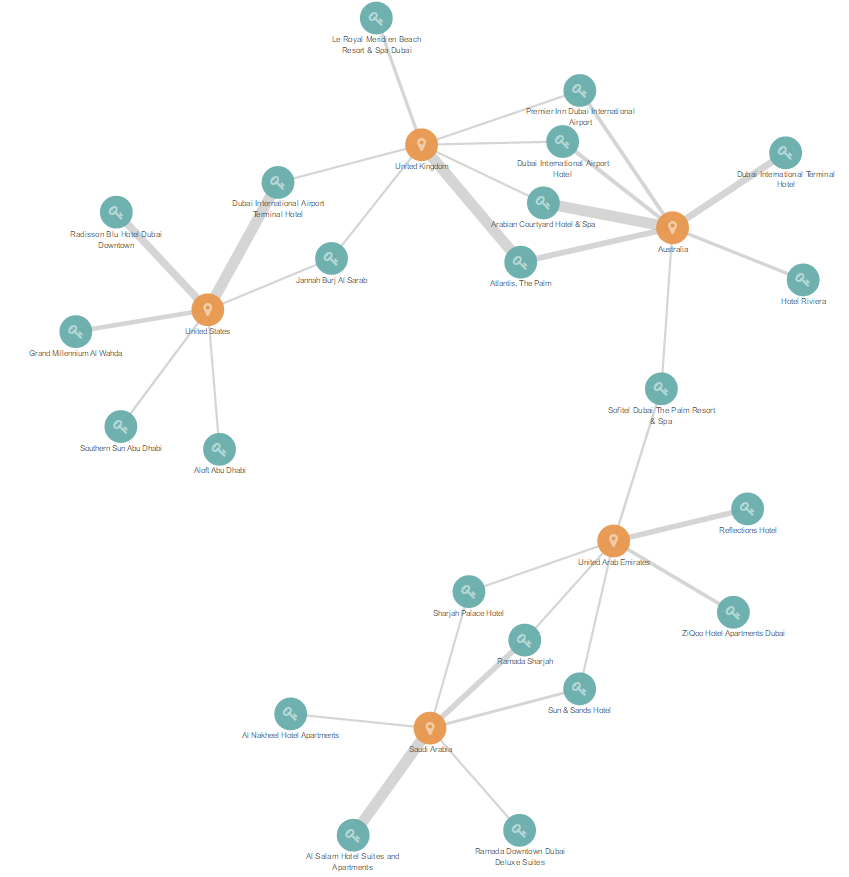
\includegraphics[width = \textwidth]{img/5_countries_highest_appearance_graph.png}
\end{center}
Z grafu lze vyčíst, že anglofonní země jakou jsou Velká Británie, Spojené státy americké nebo Austrálie preferují podobné hotely, což lze vidět především u hotelů, které mají spojení mezi Austrálií a Velkou Británií. Naopak země Arabského poloostrova, které jsou v grafu reprezentovány Saudskou Arábií a Spojenými arabskými emiráty preferují jiné hotely než anglofonní země. Zároveň však uživatelé z těchto zemí mají v oblibě podobné hotely, což značí 3 hotely, které mají spojení jak se Saudskou Arábií, tak se Spojenými arabskými emiráty. Dle mého názoru se dal takovýto výsledek na otázku očekávat a to především kvůli velikosti jednotlivých zemí, které jsou v grafu zastoupeny. Překvapivým je pro mne pouze zastoupení Austrálie, ale může to být především způsobeno geografickou polohou Dubaje, přes který míří velké množství letů z Evropy do Austrálie a opačně. To může způsobit, že většina cestujících z Austrálie stráví část dovolené právě v Dubaji, kdy čeká na navazující let do cílové destinace. To potvrzují i následující tabulka a graf, který reprezentuje zastoupení jednotlivých typů cest na celkovém počtu recenzí. Nejvýraznější zastoupení má typ cesty \uv{other}. Obě vizualizace vznikly nástrojem Kibana a jsou uložené v indexu \uv{hospitality} pod názvy Australia travel type respektive pod názvem Australia travel type table.

\begin{table}[h]
	\centering
	
	\begin{tabular}{|c|c|}
		\hline
		\multicolumn{1}{|l|}{\textbf{Roční období}} & \multicolumn{1}{l|}{\textbf{Počet nových recenzí}} \\ \hline
		Other                                        &  3340                                              \\ \hline
		Couple                                        &  2111                                            \\ \hline
		Family                                        &  1124                                              \\ \hline
		Leisure trip                                      &  945                                              \\ \hline
		Business trip                                      &  684                                              \\ \hline
		Goup                                      &  409                                              \\ \hline
		Leisure trip                                      &  191                                              \\ \hline
	\end{tabular}
\caption{Tabulka s druhy cest}
\end{table}
\begin{figure} [h]
	\centering
	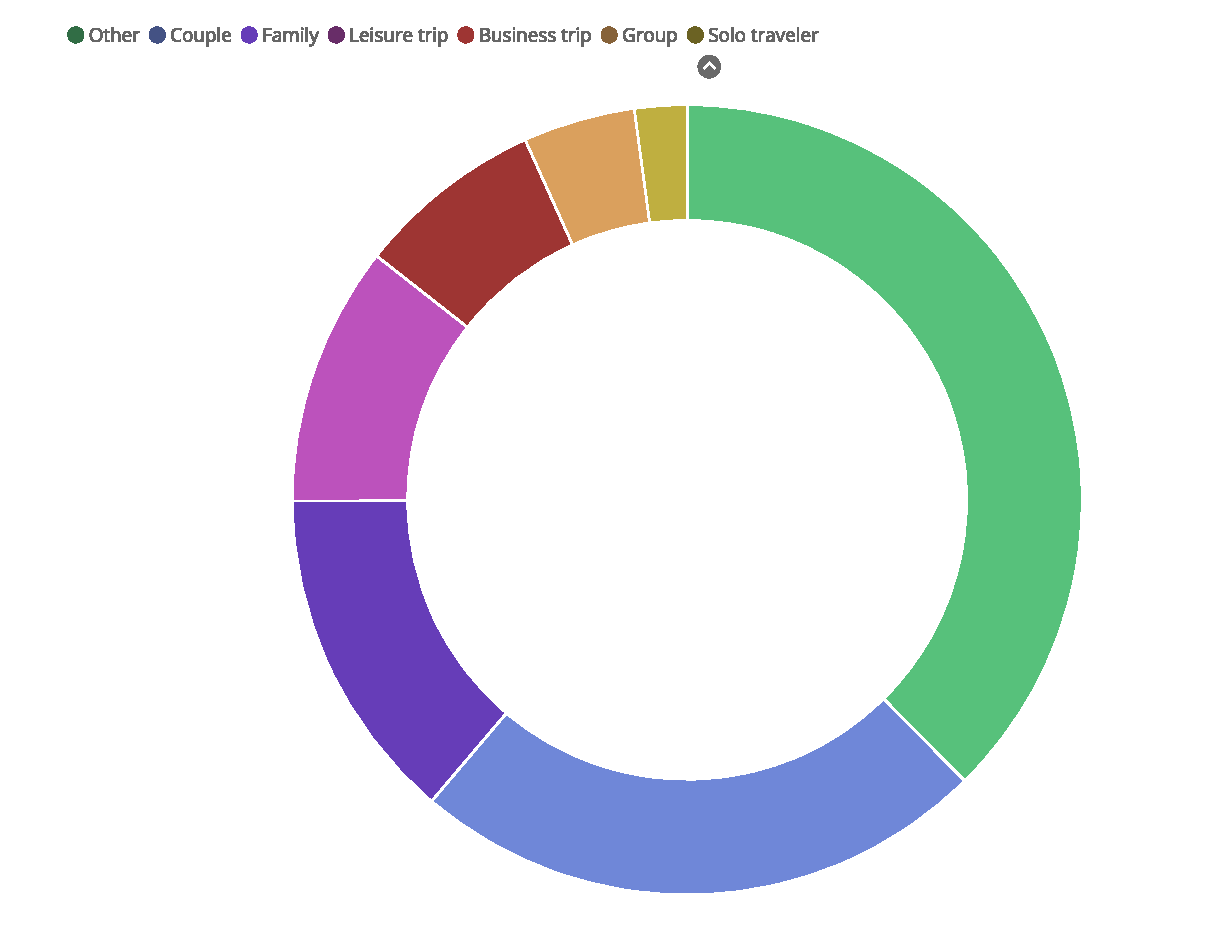
\includegraphics[width=10cm]{img/australia.eps}
	\label{Rozložení typů cest u Australanů}
	\caption{Rozložení typů cest u Australanů}
\end{figure}


Silné zastoupení zemí z Arabského poloostrova, které se umístily na druhém a třetím místě, co se do celkového počtu recenzí týče, je zapříčiněno geografickou polohou, jelikož se jedná o velmi blízké sousedy Dubaje, v případě Spojeným arabských emirátů se jedná dokonce o hlavní město stejnojmenného emirátu.


Velmi zajímavé je na výsledném grafu sledovat sílu jednotlivých spojení, která je symbolizována tloušťkou čáry mezi jednotlivými vrcholy grafu. Jelikož je výsledný graf fakticky složený z více výsledků hledání spojení, je irelevantní porovnávat sílu spojení mezi hotely a různými zeměmi. To je možné zpozorovat pří porovnání šířky spojení mezi hotelem \uv{Atlantis, The Palm} a zeměmi Velká Británie a Austrálie. Detail tohoto spojení lze vidět na následujícím obrázku.

\begin{center}
	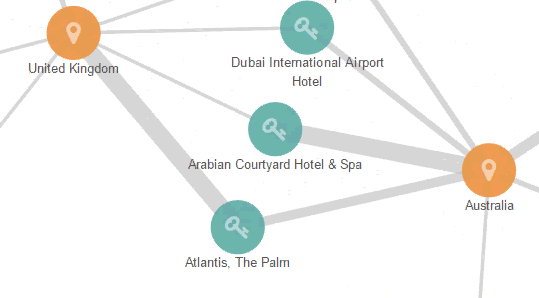
\includegraphics[width=\textwidth]{img/detail_spojeni.PNG}
\end{center}

 Na první pohled by se mohlo zdát, že do téhož hotelu jezdí zhruba dvojnásobné množství hostů z Velké Británie než hostů z Austrálie, ale ve skutečnosti je poměr větší. Hlavní příčinou je \uv{spidering}, který sice přidá spojení mezi existujícími vrcholy, ale nebere v potaz již existující spojení, které do těchto vrcholů vedou. Další příčinou je samostatný princip rozšíření Graph, který určuje sílu spojení mezi vrcholy ne podle poměru počtu dokumentů, kde se vyskytují oba výrazy ku celkovému počtu dokumentů, ale závisí jen na poměru počtu dokumentů, kde se vyskytují oba výrazy ku počtu dokumentů, kde se vyskytuje alespoň jeden z výrazů. Jedná se tedy vlastně o průnik množiny dokumentů, které obsahují výraz A a množiny dokumentů, které obsahují výraz B. Abychom tedy zjistili reálnou sílu spojení, je nutné kliknout na jednotlivá spojení a získat detailnější informace. Tyto informace jsou zjistitelné z následujících obrázků.

\begin{center}
	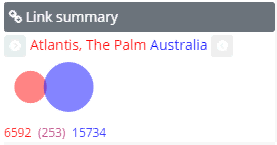
\includegraphics[scale=0.85]{img/AUS_atlantis.PNG}
	\hspace{0.4cm}
	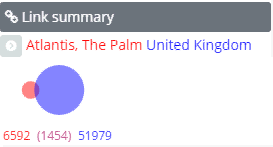
\includegraphics[scale=0.85]{img/UK_atlantis.PNG}
\end{center}


Červená čísla na obrázcích reprezentují počet dokumentů, které obsahují v poli HOTEL\_NAME.keyword hodnotu \uv{Atlantis, The Palm}, modrá čísla reprezentují na horním obrázku počet recenzí, které obsahují v poli U\-SER\_LOCATION\_COUNTRY.keyword hodnotu Australia a na spodním obrázku recenze obsahující v témže poli hodnotu United Kingdom. Růžová čísla reprezentují průnik množin, a jak je možné vidět, tentýž hotel je přibližně sedm krát častěji recenzován uživateli z Velké Británie než uživateli z Austrálie, což je oproti původnímu odhadu velký rozdíl.

\subsubsection{Charakterizujte návštěvníky hotelů, kteří jezdí do Dubaje na pracovní cesty, dovolenou, líbánky a podobně.}
\label{subsub:Charakteristika návštěvníků}
Ke zpracování této otázky je taktéž vhodné využít rozšíření Graph, protože hledáme spojitosti mezi typem cest a charakteristickými rysy návštěvníků. Těmito rysy je například stát, věk návštěvníků nebo pozitiva, která návštěvníci zmínili ve svých recenzích. Jelikož je v otázce požadováno určit charakteristiky pro jednotlivé typy cest, je nutné vytvořit více samostatných vizualizací. Tyto vizualizace odpovídají vždy danému typu cesty.


Problémem při hledání odpovědí byla stejně jako v předchozí otázce neúplná data. Z toho důvodu je možné charakterizovat pouze návštěvníky, kteří se vydali buďto na pracovní cestu, nebo na dovolenou. Data od uživatelů, kteří byli na líbánkách, nebo na výletě nejsou z recenzí k dispozici. Odpovědi jsou také ovlivněny vlastností nástroje Graph, v jehož výstupu jsou vrcholy s největším ohodnocením. To je také důvod, proč jsou země v odpovědích rozdílné od zemí, které jsou zastoupeny v předchozí otázce.

\paragraph{Charakteristika obchodních cestujících}
\mbox{}\\
Na obrázku \ref{fig:Business} je vidět charakteristika návštěvníků Dubaje, kteří přijeli na pracovní cestu. Z vizualizace je patrné, že jsou návštěvníci rozděleni do třech věkových skupin, u kterých se liší především země, ze kterých obchodní cestující pocházejí. Jedná se o skupiny lidí ve věku 35-44, 45-54 a 55-64 let. Lidé patřící do těchto skupin jsou tedy v produktivním věku. Z toho, že chybí skupina 24-35 let, lze vyvodit, že do Dubaje jezdí především zkušení zaměstnanci či obchodníci. Dle mého názoru chybí tato skupina z důvodu, že se v Dubaji uzavírají obchody především ve finančním sektoru. V tomto sektoru je vyžadována po zaměstnancích zkušenost a také vysoké vzdělání. To že je Dubaj centrem ochodu potvrzují budovy, jako jsou World Trade Center, Financial Centre, Business Bay. Nejen však tyto budovy, ale i fakt, že Dubaj byla v roce 2015 vyhlášena nejvýznamnějším obchodním centrem světa.\cite{BusinessDubai} 


Není překvapením, že jsou v silném zastoupení země Arabského poloostrova a to především ve věkových skupinách 35 až 44 let a 45 až 54 let. Důvodem tohoto silného zastoupení je samozřejmě geografická poloha Dubaje a jeho vzdálenost od zemí, které jsou ve vizualizaci zastoupeny. Jak již bylo zmíněno, je Dubaj celosvětově významným obchodním centrem, takže není překvapivé značné zastoupení okolních zemí ve vizualizaci. Pro firmy z těchto zemí je Dubaj hlavním centrem podnikání, takže do města vysílají své zaměstnance, kteří se při té příležitosti mohou ubytovat v místních hotelech.


Pro věkovou skupinu 55 až 64 let jsou typické země Mauricius, Kypr a Řecko. První dvě jmenované země nejsou pro mne překvapením, protože zde mají své rezidence movití lidé z finančního sektoru. Mauricius si tito lidé vybírají především kvůli geografické poloze a klimatickým podmínkám. Kypr je známý daňový ráj díky svým nízkým daním, tudíž není divu, že movití lidé na Kypr přesouvají svá sídla a také sídla svých firem. Překvapením pro mne je pouze výskyt Řecka ve výsledné vizualizaci. Je možné, že je to způsobené kombinací polohy, klimatu a také přístupu Řecka k výběru daní. Řecký ukazatel vymahatelnosti daní klesl od roku 2010 o 20 procentních bodů na 50 procent, což je 35 procentních bodů horší než Malta, která je druhá nejhorší ve výběru daní v zemích Evropské unie.\cite{GreeceTaxes} 


Obecně lze říci, že hlavním pozitivem, které shledávají všechny tři věkové skupiny, je lokace hotelu a servis, který je v hotelu poskytován. Dále je pro skupiny 35-44 let a 45-54 let důležitá čistota hotelů.
\begin{figure}[htbp]
	\centering
	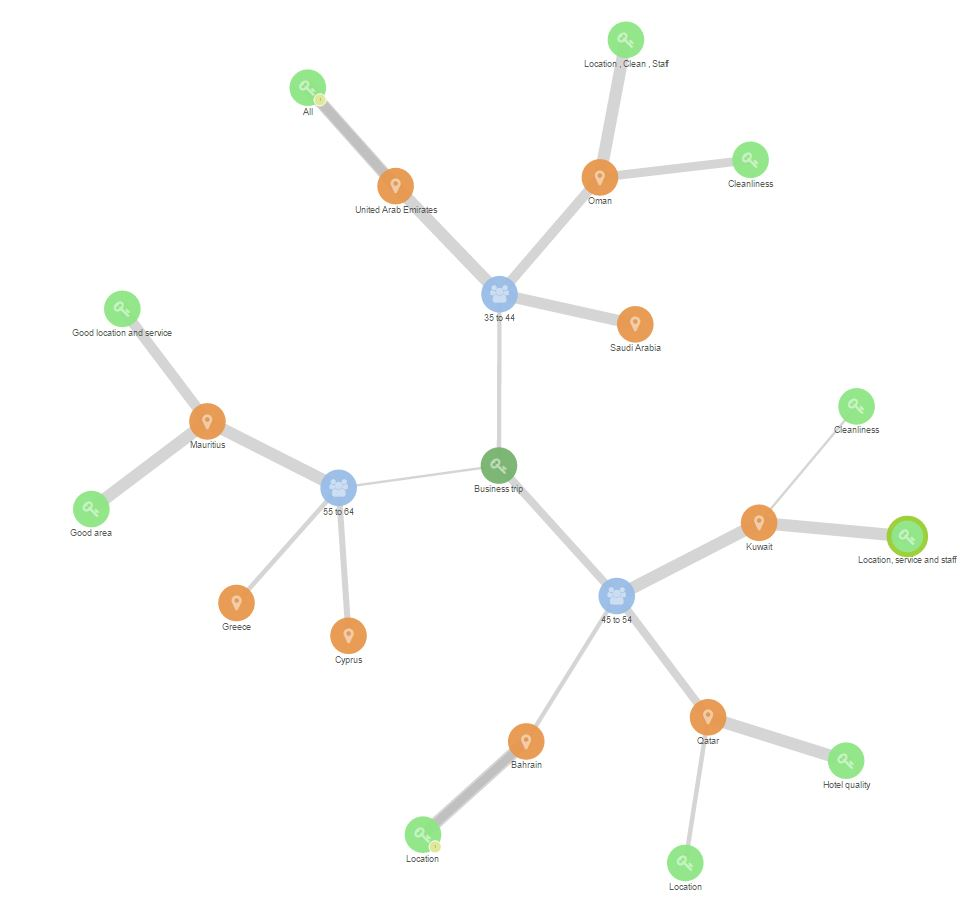
\includegraphics[width = 10cm]{img/Business_trip_customers_proportions.jpg}
	\caption{Charakteristika obchodních cestujících.}
	\label{fig:Business}	
\end{figure}


\paragraph{Charakteristika lidí jezdících do Dubaje na dovolenou}
\mbox{}\\
Na obrázku \ref{fig:Leisure} je k vidění charakteristika návštěvníků, kteří přijeli do Dubaje strávit svůj volný čas. Z vizualizace je patrné, že i zde jsou návštěvníci rozděleni do třech věkových kategorií. Na rozdíl od obchodních cestující je zde výrazněji zastoupena skupina 25-34 let a to na úkor věkové skupiny 55-64 let. Dle mého názoru je to způsobeno vyšším věkem nahrazené skupiny, se kterým přicházejí zdravotní problémy. Z tohoto důvodu bych tuto skupinu očekával především u ozdravných pobytů, o kterých máme ovšem nedostatek dat. Ve vizualizaci jsou tedy zastoupeny věkové skupiny 25-34, 35-44 a 45-54 let.

\begin{figure}[htbp]
	\centering
	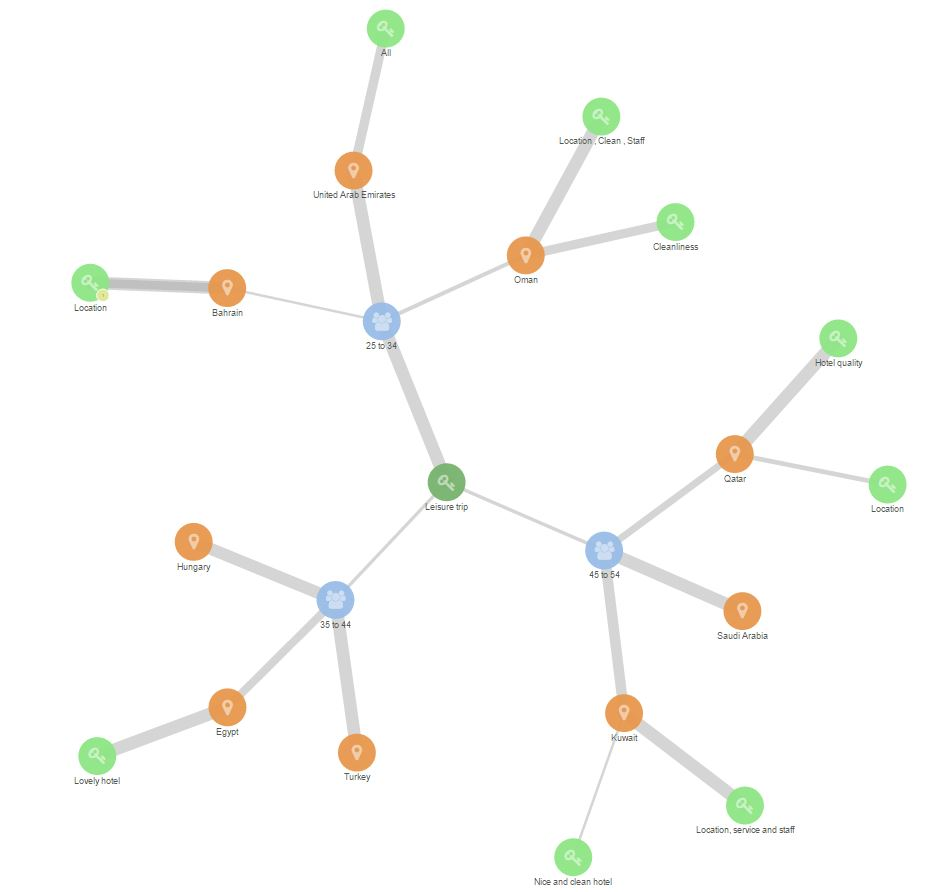
\includegraphics[ width = 10.5cm]{img/Leisure_trip_customers_proportions_cut.jpg}
	\caption{Charakteristika lidí na dovolené.}
	\label{fig:Leisure}	
\end{figure}


Ve věkových skupinách 25-34 a 45-54 jsou zastoupeny pouze státy, které se nacházejí na Arabském poloostrově. Způsobeno je to dle mého názoru nejen geografickou polohou, ale také finanční náročností. Ta je pro občany zastoupených států menší než pro ostatní země z jiných kontinentů, protože ušetří na nákladech na dopravu. Letecká doprava ze zemí Arabského poloostrova do Dubaje je určitě levnější, než letecká doprava z jiných zemí na světě. Tyto důvody hrají dle mého názoru roli především pro věkovou skupinu 25-34 let. Pro skupinu 45-54 let může být rozhodující také časová náročnost dopravy a s tím související fyzická náročnost dopravy.


Prostřední věková skupina je velkým překvapením, jelikož jsou zde zastoupeny netypické země. Dle mého názoru je to způsobeno menším počtem recenzí, které uživatelé z těchto zemí napsali. Také fakt, že část recenzí nemá pole USER\_AGE\_GROUP, mohl způsobit výskyt těchto zemí. Dále výsledek ovlivnil nástroj Graph svým specifickým výběrem vrcholů podle jejich ohodnocení. 


Stejně jako u lidí na obchodních cestách je i u lidí na dovolených důležitá lokace hotelu, jeho služby a čistota. To lze vypozorovat z nejčastějších pozitiv, které zanechali návštěvníci ve svých recenzích.


Výstup této otázky je možné využít především pro marketingové účely. Hotely mohou zaměřit své reklamy na specifické věkové skupiny a navíc mají nyní přehled, z jakých zemí k nim tyto skupiny přijíždějí. Například mohou využít reklamu na sociálních sítích pro země, ze kterých jezdí návštěvníci z nejmladší věkové skupiny.

\paragraph{Postup při tvorbě vizualizace}
\mbox{}\\
V první řadě je v nástroji Graph nutné zvolit index, v jehož dokumentech bude nástroj provádět hledání. Dále si je nutné zvolit vhodné výrazy, pomocí kterých nástroj Graph hledá spojení mezi vybranými zdrojovými poli. Tyto výrazy obsahuje pole TRAVEL\_TYPE, ale ne všechny výrazy mají v dokumentech zastoupení v dostatečné míře, takže například pro výraz \uv{Couple} není nalezen žádný vrchol. Je možné zadat jen výrazy \uv{Business trip} a \uv{Leisure trip}. Jako zdrojová pole zvolím pole USER\_AGE\_GROUP, nastavím počet vrcholů z tohoto pole na tři a spustím nástroj Graph s patřičným výrazem ve vyhledávacím poli. Výsledkem je jednoduchý kruhový graf, v jehož středu je vrchol odpovídající výrazu z vyhledávacího pole a na něj jsou navázány celkem tři různé věkové skupiny.


Dále chceme zpřesnit charakteristiku jednotlivých skupin o země, ze kterých nejčastěji návštěvníci jezdí. Ponecháme tedy výraz z původního hledání ve vyhledávacím poli, zneaktivníme zdrojové pole USER\_AGE\_GROUP a přidáme nové zdrojové pole USER\_LOCATION\_COUNTRY, které obsahuje domovské státy recenzentů. U tohoto pole nastavíme, že požadujeme pouze tři výsledné vrcholy reprezentující země. Nyní je nutné rozšířit výsledný graf, což se provede označením vybrané věkové skupiny a stiskem tlačítka \uv{Add links}. Po provedení procesu \uv{spidering} pro všechny skupiny uživatelů, které byly zastoupeny v původní jednoduché vizualizaci, se nová vizualizace skládá celkem ze tři úrovní a to z typu cesty, věkové skupiny a zemí, ze kterých pocházejí recenzenti.


Posledním krokem k získání vizualizace, kterou můžete vidět na obrázcích \ref{fig:Business} a \ref{fig:Leisure} je přidání pozitivních výrazů, které recenzenti zanechali. Přidáme pole POSITIVE.keyword, zneaktivníme i pole USER\_LOCATION\_COUNTRY a postupně rozšíříme jednotlivé země o nejčastější hodnoty z pole POSITIVE.keyword. Rozšíření provádíme obdobným způsobem jako při rozšiřování grafu o země uživatelů. Může se stát, že nově vzniklé vrcholy budou u stejných zemí obsahovat duplicitní hodnoty. Tyto vrcholy můžeme následně sloučit pomocí tlačítka \uv{Group}. Pokud je vrchol složen z vícero vrcholů, zobrazí se na výsledné vizualizaci u tohoto vrcholu žlutě vyplněný kruh.

\section{Nástroje Kibana}
\subsubsection{Jaká je sezóní návštěvnost Dubaje podle států?}
\label{subsub:Návštěvnost}
\paragraph{Použité nástroje}
\mbox{}\\
K zodpovězení této otázky jsem využil data o vzniku recenzí, které se nacházejí v poli DATE\_CREATED. Jelikož jsou tato data rozdělena podle roků, byla by vizualizace odpovědi nepřehledná, takže jsem se rozhodl pro lehkou modifikaci dostupných dat. Modifikace spočívá ve vytvoření nového pole DATE\_CREATED\_SEASONS, ve kterém se nacházejí data z pole DATE\_CREATED, ale všechna data mají nastavený rok 2000. Tuto modifikaci provedl vedoucí této práce. Aby nedošlo ke zkreslení hodnot v indexu \uv{hospitality}, tak jsem vytvořil nový index \uv{new\_index}, z jehož dat jsem tvořil vizualizaci odpovědi. Lepší variantou by bylo využít data z pole STAYED, ale bohužel nejsou hodnoty v tomto poli u většiny recenzí vyplněné. 


Při vizualizaci jsem využil nástroje, které poskytuje Kibana již v základu. Konkrétně se jedná o výsečový graf, který jsem využil k zobrazení rozložení návštěvnosti mezi jednotlivá roční období. Dále jsem využil graf liniový, jenž je vhodný k vizualizaci rozložení návštěvnosti jednotlivých národností mezi roční období.

\paragraph{Odpověď na otázku}
\mbox{}\\
Otázka požaduje zobrazení sezónní návštěvnosti Dubaje podle států, ale dle mého názoru je nejprve důležité vizualizovat obecné rozložení návštěvnosti všech návštěvníků. Díky této vizualizaci poté bude možné porovnávat globální trend s trendy jednotlivých států.
\vspace{2cm}
\paragraph{Globální rozložení návštěvnosti do sezón}\mbox{}\\
V grafu \ref{fig:Pie_global_visitors} je možné vidět procentuální zastoupení jednotlivých ročních období na celkové návštěvnosti Dubaje. Je vidět, že destinace je oblíbená celoročně a kromě jara je návštěvnost rozdělena mezi jednotlivá období celkem rovnoměrně. Jaro mírně vybočuje, ale pouze o 2 - 3 procentní body. Toto rovnoměrné rozdělení je dáno především místním klimatem, jelikož je průměrná roční teplota $\SI{27.8}{\degreeCelsius}$.\cite{DubaiTemperature}Průměrné teploty v jarních měsících se pohybují mezi 28 - $\SI{36}{\degreeCelsius}$ a teplota moře v těchto měsících je v rozmezí 24 - $\SI{27}{\degreeCelsius}$. Právě kvůli těmto údajům je jaro u návštěvníků oblíbenější, než ostatní roční období. V létě dosahují totiž teploty vzduchu až $\SI{45}{\degreeCelsius}$ a moře má teplotu až $\SI{38}{\degreeCelsius}$. Podzim a zima mají obdobné teploty vzduchu jako jaro, ale moře má teplotu nižší.

\begin{figure}[htbp]
	\centering
	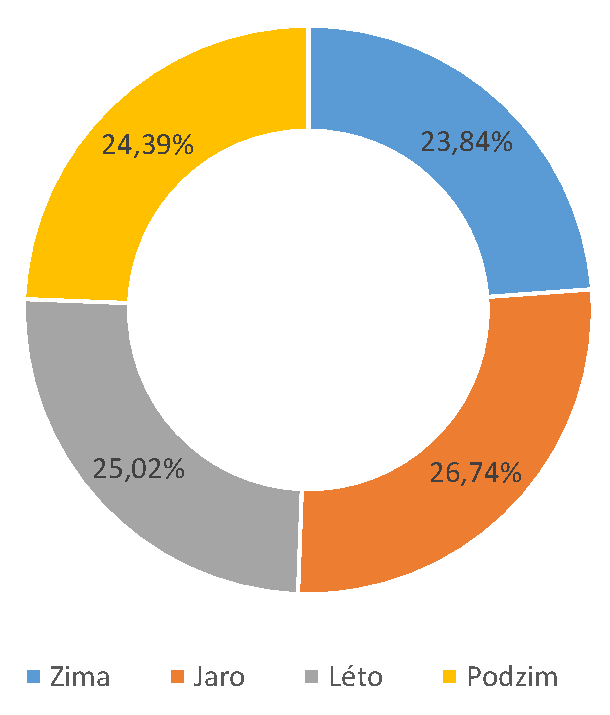
\includegraphics[ width = 5cm]{img/rocni_donut.eps}
	\caption{Rozložení návštěvnosti do sezón}
	\label{fig:Pie_global_visitors}	
\end{figure}

V následující tabulce je vidět počet přidaných recenzí pro jednotlivá roční období.

\begin{table}[h]
	\centering
	
	\begin{tabular}{|c|c|}
		\hline
		\multicolumn{1}{|l|}{\textbf{Roční období}} & \multicolumn{1}{l|}{\textbf{Počet nových recenzí}} \\ \hline
		ZIMA                                        & 87 493                                              \\ \hline
		JARO                                        & 100 602                                             \\ \hline
		LÉTO                                        & 91 817                                              \\ \hline
		PODZIM                                      & 89 512                                              \\ \hline
	\end{tabular}
\caption{Počet přidaných recenzí za roční období}
\label{Recenze celkem}
\end{table}

\paragraph{Sezónní rozložení návštěvnosti podle států}\mbox{}\\
Do vizualizace jsem zahrnul data pěti států, ze kterých pochází nejvíce recenzí. Liniový graf \ref{fig:Sezona_staty} zobrazuje trendy návštěvníků z těchto států a jejich oblíbená roční období. V pravé části grafu dochází k výraznému poklesu křivek, ale je to způsobené zvoleným časovým intervalem, který obsahuje data jen za deset dní. Jelikož jsou všechna data v poli DATE\_CREATED\_SEA- SSONS datována do roku 2000, nelze zvolit lepší časový interval. Rovnoměrné rozložení návštěvnosti je dáno především rozdílnými trendy mezi západními státy, které jsou reprezentovány Spojeným královstvím a Spojenými státy americkými, a mezi východními státy, jež ve vizualizaci reprezentují Spojené arabské emiráty, Saudská Arábie a Austrálie. U západních států dochází v jarních a letních měsících k lehkému poklesu, ale u východních zástupců dochází k přesnému opaku.


Z grafu je patrné, že nejoblíbenější měsíce pro návštěvníky ze Spojeného království a ze Spojených států patří březen a listopad. Mezi těmito měsíci dochází k poklesu návštěvnosti, což je nejspíše důsledek vyšších teplot, které v Dubaji panují. Lze usoudit, že návštěvníci z těchto států jezdí do Dubaje nejčastěji od podzimu až do března a ve zbytku roku počet návštěvníků klesá.


Tendence návštěvníku ze zemí Arabského poloostrova a z Austrálie jsou opačné tendencím západních zemí. Jelikož jsou obyvatelé z těchto zemí zvyklí na teplé podnebí, má křivka návštěvnosti vrchol v létě a v ostatních ročních obdobích jejich návštěvnost klesá.




\begin{figure}[htbp]
	\centering
	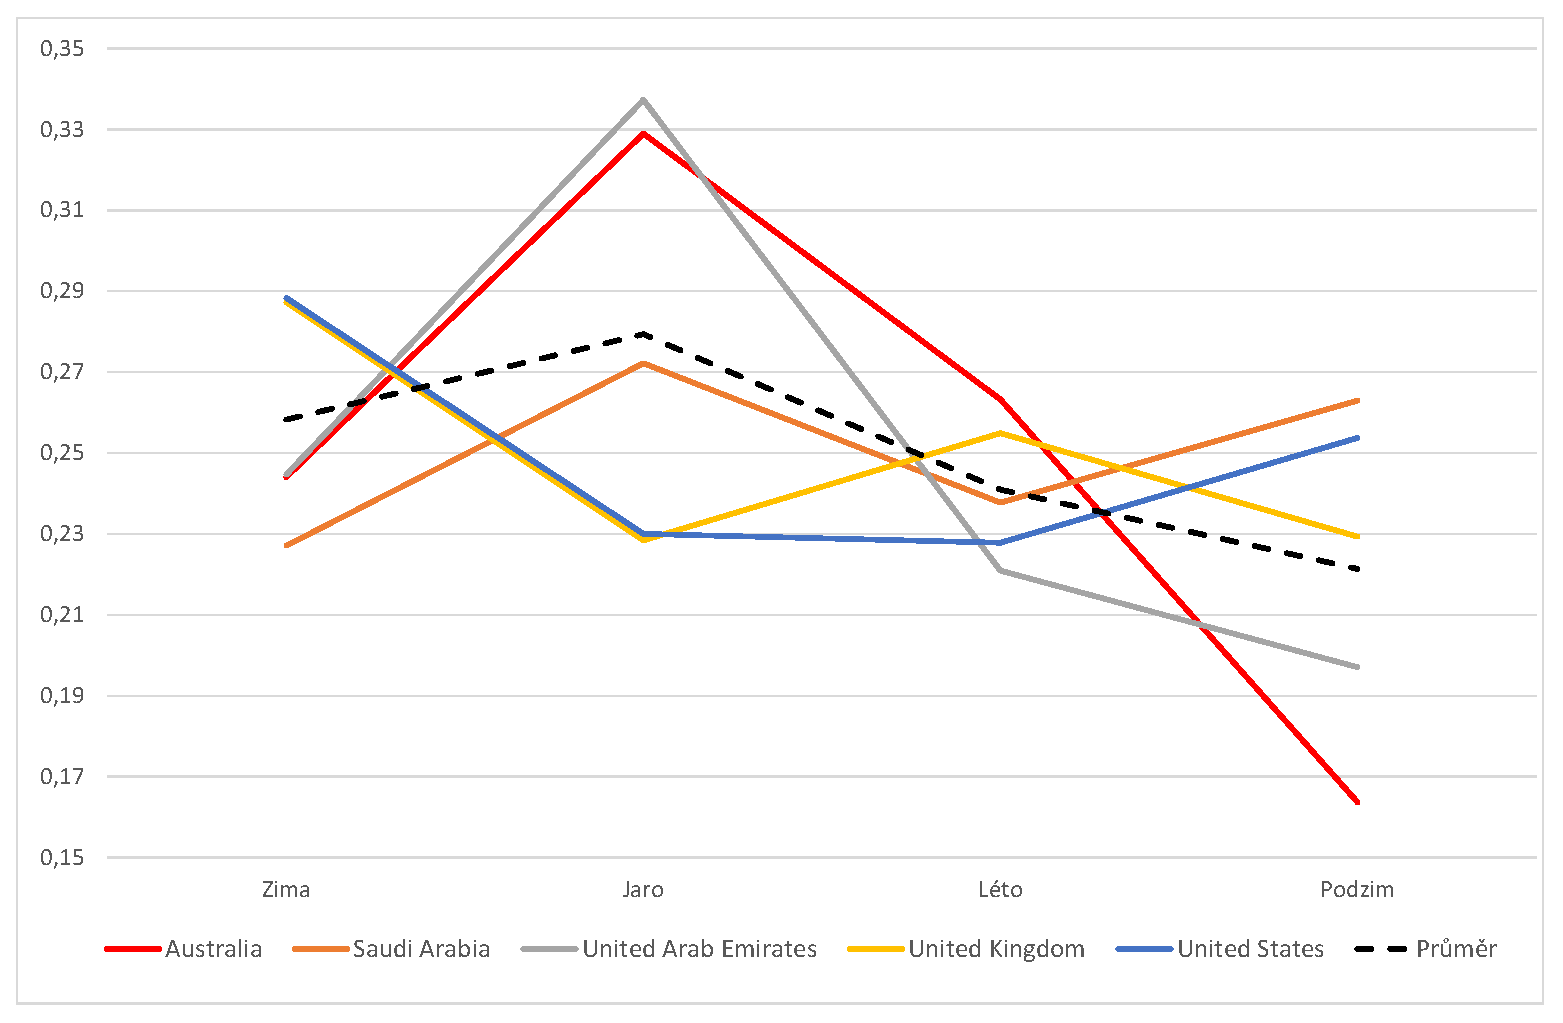
\includegraphics[ width = \textwidth]{img/graf_sezona.eps}
	\caption{Sezónní vývoj návštěvnosti podle států}
	\label{fig:Sezona_staty}	
\end{figure}\textbf{}

\paragraph{Postup při tvorbě vizualizace odpovědi}
\mbox{}\\
Jak již bylo zmíněno, využil jsem dva typy grafů a to koláčový pro globální trendy v návštěvnosti a liniový pro trendy jednotlivých zemí. Koláčový graf je jednoduchý a stačí vyplnit jen agregaci \uv{Date Range}, zdrojové pole DATE\_CREATED\_SEASONS a následně vyplnit meze podle ročních období. Důležité je, že se musí zvolit celkem 5 mezí, protože jsou všechny data koncipována do roku 2000, takže nelze jasně vymezit zimní období, protože obsahuje přelom roku.


Ani liniový graf není obtížný. Na ose y je počet recenzí, které byly v daném období přidány a na ose x jsou jednotlivá období. Agregace na ose x je stejná jako u koláčového grafu. Dále je nutné přidat jednotlivé země, což se provede kliknutím na \uv{Add sub-buckets} a volbou \uv{Split Lines}. Ve \uv{Split Lines} zvolíme agregaci podle výrazů a jako zdrojové pole vybereme USER\_LOCATION\_COUNTRY.keyword. Počet zemí omezíme na 5 a volíme sestupné řazení. Výsledek vizualizace bude ovšem matoucí, protože se zobrazí celkem 6 zemí i přes omezení výsledků na 5. Zároveň se zkreslí data pro Austrálii, kdy údajně nepřibyly žádné recenze v zimních měsících. Jedná se nejspíše o interní chybu nástroje Kibana a je nutné ji vyřešit pomocí filtrů. Postupně se musí zakázat výskyt Irska a Indie. Po vyfiltrování již vzniklá vizualizace odpovídá vizualizaci \ref{fig:Sezona_staty}.

\subsubsection{Jak hodnotí návštěvníci jídlo nabízené v hotelích?}
\label{subsub:Jídlo}
Odpověď na tuto otázku lze získat z dostupných dat celkem snadno, protože je v datech k dispozici pole SENTIMENT\_FOOD. Pole v datech, která začínají slovem SENTIMENT, vznikla z analýzy sentimentu, která byla provedena nad texty všech recenzí. Analýza sentimentu je součástí zpracování přirozeného jazyka, čímž se skupiny NLP zabývá. Tato pole obsahují hodnoty 1, 0 nebo -1, přičemž -1 značí nespokojenost a 1 naopak spokojenost. Právě díky dostupnosti těchto dat je možné vyjádřit spokojenost s jídlem jako průměrnou hodnotu pole SENTIMENT\_FOOD. Tato hodnota je graficky i číselně vyjádřena na obrázku \ref{fig:Food_sentiment}. Na obrázku je vidět také číslo, které odpovídá celkovému počtu recenzí, ve kterých bylo jídlo hodnoceno. Jedná se celkem o 20,59\% všech recenzí, což je vzhledem k úplnosti dat celkem přijatelný výsledek. Z vizualizace je vidět, že jsou hodnotící zákazníci s jídlem spokojení a převažují kladné pocity nad negativními.

\begin{figure}[h]
	\centering
	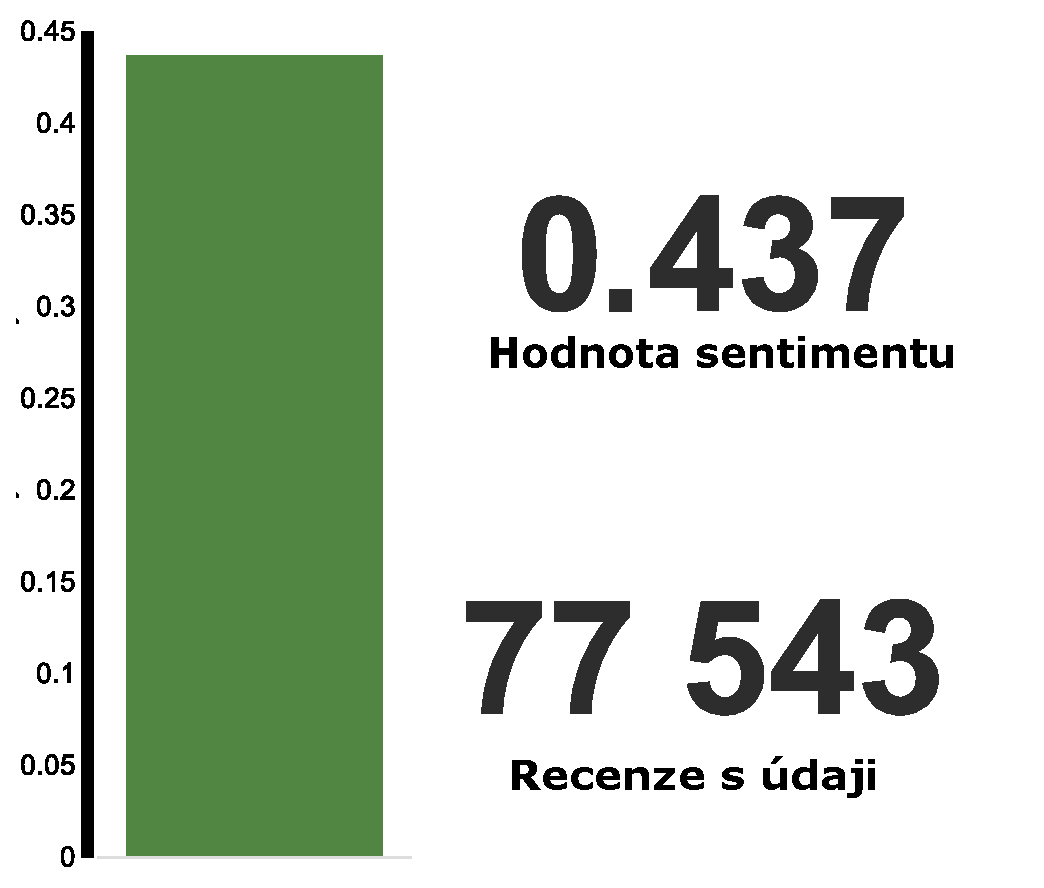
\includegraphics[ width =8cm]{img/food.eps}
	\caption{Spokojenost hostů s jídlem}
	\label{fig:Food_sentiment}	
\end{figure}


Na obrázku \ref{fig:Food_tags} jsou k vidění nejčastější fráze, které byly použity v recenzích hodnotící jídlo. K vizualizaci byl použit nástroj \uv{Tag cloud}, který je dostupný již v základní verzi nástroje Kibana. Při tvorbě bylo použito pole POSITIVE.keyword a ve vyhledávacím poli jsem použil dotaz ve tvaru \uv{POSITIVE.keyword:*FOOD}.
\begin{figure}[h]
	\centering
	
\includegraphics[ width = 8cm]{img/food_positive.eps}
	\caption{Slovní hodnocení jídla}
	\label{fig:Food_tags}	
\end{figure}

\subsubsection{Je přínos z cesty do Dubaje úměrný vynaloženým nákladům?}
\label{subsub:Worth of money}
Odpověď na otázku lze získat přímo z dat bez nutnosti jejich úpravy. Data obsahují pole X\_SCORE\_VALUE\_FOR\_MONEY, kde je uložené skóre jednotlivých uživatelů, kteří se vyjádřili k přínosům cesty a nákladům na ní. Platí, že čím vyšší je hodnota v tomto poli, tím více se jim vynaložené náklady na cestu zdají adekvátní k přínosům. Na obrázku \ref{fig:Worth_of_money} je zobrazena maximální, minimální a průměrná hodnota pole X\_SCORE\_VA- LUE\_FOR\_MONEY a zároveň je na obrázku číslo udávající počet recenzí, které mají vyplněné hodnoty v tomto poli. Lze konstatovat, že jsou návštěvníci s náklady na cestu převážně spokojení a výsledky lze považovat za relevantní, protože vycházejí ze 48,9\% všech dostupných recenzí.

\begin{figure}[htbp]
	\centering
	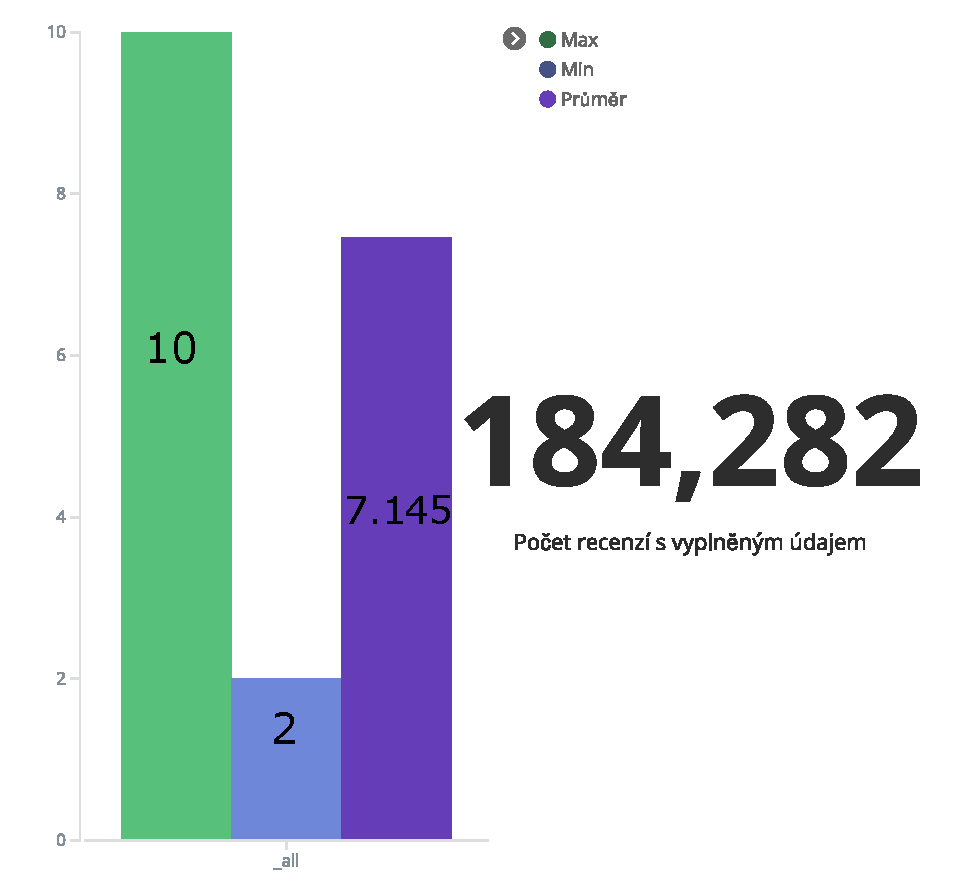
\includegraphics[ width = 10cm]{img/worth_money.eps}
	\caption{Přínos z cesty}
	\label{fig:Worth_of_money}	
\end{figure}

\subsubsection{Jak hodnotí návštěvníci kvalitu služeb?}
\label{subsub:služby}
Odpovědi na otázku lze hledat také přímo v recenzích, které máme k dispozici. Konkrétně jsou klíčové hodnoty uložené v polích REVIEW\_SCO- RE\_SERVICE, SCORE\_SERVICE\textbackslash STAFF a SENTIMENT\_SERVICE.\\ Hodnoty z prvního pole vyjadřují spokojenost jednotlivých návštěvníků se službami, které hotel poskytuje. Mezi tyto služby patří například pokojový servis, připojení k internetu, kvalita hotelových bazénů, nebo doprovodné programy. Průměrná hodnota v tomto poli je 9,133, což značí, že jsou návštěvníci s kvalitou poskytovaných služeb velmi spokojeni. Nižší průměrnou hodnotu obsahuje pole SCORE\_SERVICE\textbackslash STAFF, které kromě poskytovaných služeb také hodnotí přístup personálu a jejich ochotu. Jelikož je průměrná hodnota nižší než průměrná hodnota pole REVIEW\_SCORE\_SER- VICE, lze usoudit, že návštěvníci spatřují v personálu slabé místo, na které by se měly hotely zaměřit. Průměrné hodnoty z těchto dvou polí by měly být co nejvíce podobné, ideálně stejné. Třetí sloupec na obrázku \ref{fig:Services} ukazuje průměrnou hodnotu v poli SENTIMENT\_SERVICE. Z kladné hodnoty průměrného sentimentu lze vyvodit celkovou spokojenost s kvalitou poskytovaných služeb, čímž jsme potvrdili výsledky průměrných hodnot v polích REVIEW\_SCORE\_SERVICE a SCORE\_SERVICE\textbackslash STAFF. Odpověď na otázku vychází z 31,54\% všech dostupných recenzí, takže lze výsledky prohlásit za relevantní.
% 

\begin{figure}[htbp]
	\centering
	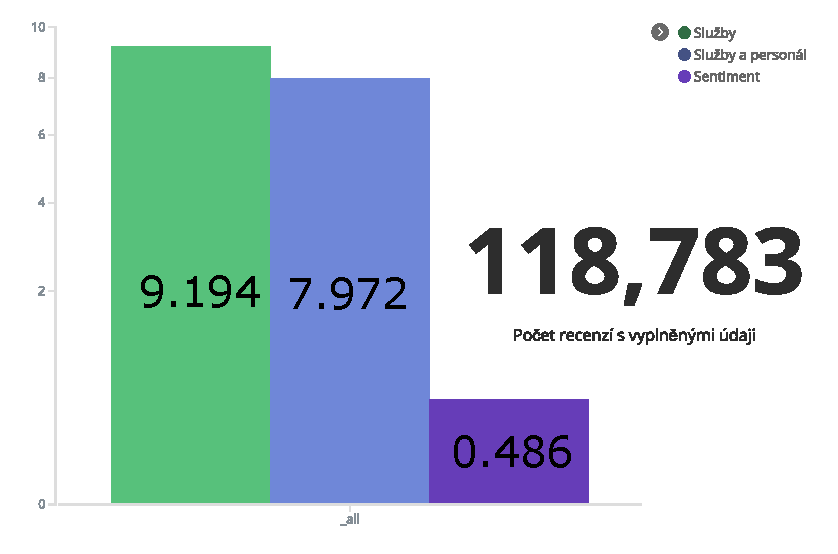
\includegraphics[ width = 10cm]{img/sluzby.eps}
	\caption{Kvalita služeb}
	\label{fig:Services}	
\end{figure}



Mezi nejčastěji hodnocené služby patří internetové připojení, které je v dnešní době velmi důležité především pro obchodní cestující. Hotely poskytují připojení prostřednictvím WiFi připojení, které je buďto zdarma, nebo je zpoplatněno. Předpokládám, že hotely nejčastěji poskytují připojení zdarma, protože pole X\_SCORE\_FREE\_WIFI obsahuje 103 804 záznamů, ale pole X\_SCORE\_PAID\_WIFI obsahuje pouze 8 888 záznamů. Právě velký rozdíl mezi počtem záznamů v obou polích je dle mého názoru také příčinou markantního rozdílu mezi průměrnými hodnotami v jednotlivých polích. Lépe hodnoceno je připojení zdarma a to o 2,3 bodu oproti zpoplatněnému připojení. S připojením  zdarma panuje podle recenzí spokojenost, ale hodnocení placeného připojení je spíše průměrné. Na první pohled je překvapivý je záporný sentiment u WiFi připojení, který má hodnotu -0,382. Tento výsledek se ovšem nedá brát jako relevantní, protože pole SENTIMENT\_WIFI obsahuje pouze 14 992 záznamů, což jsou pouhá 4\% dostupných recenzí. Na vizualizaci \ref{fig:WiFi} lze tedy také vidět průměrné hodnoty polí X\_SCORE\_FREE\_WIFI a X\_SCORE\_PAID\_WIFI, které obsahují celkem 108 754 záznamů, což je 28,88\% všech sebraných recenzí.

\begin{figure}[h]
	\centering
	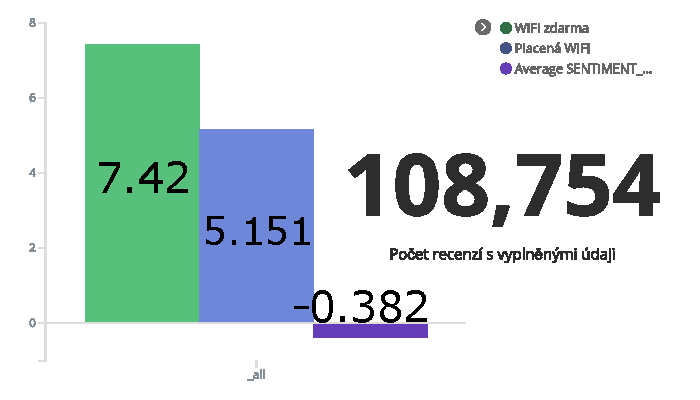
\includegraphics[ width =10cm]{img/wifi.eps}
	\caption{Hodnocení spokojenosti s internetovým připojením}
	\label{fig:WiFi}	
\end{figure}

\subsubsection{Má na návštěvníky dopad stav a čistota hotelu?}
\label{subsub:Stav a čistota}
Přesnou odpověď na tuto otázku nelze získat vizualizací přímo z dat. Vizualizovat lze pouze průměrnou hodnotu pole SCORE\_TOTAL, kde jsou uložena celková hodnocení hotelů, a pole SCORE\_HOTEL\_CONDITION/CLEAN- LINESS. Z výsledné vizualizace by ale nebylo možné vyvodit žádné relevantní výsledky, protože neznáme vztah mezi hodnotami v obou polích.


K určení vztahu mezi hodnotami ve dvou polích a ke zjištění, jak se hodnoty ovlivňují, slouží statistická metoda zvaná korelace. Výsledkem korelace je korelační koeficient, který může nabývat hodnot -1 až 1. Hodnoty korelačního koeficientu blízkého -1 značí takzvanou antikorelaci, která značí nepřímou závislost mezi hodnotami. To znamená, že pokud se zvětší hodnota v poli A, tak se hodnota v poli B adekvátně zmenší. Pokud je korelační koeficient blízký hodnotě 1, tak jsou hodnoty na sobě přímo závislé, neboli pokud se zvýší hodnota v poli A, zvýší se úměrně i hodnota v poli B. Korelační koeficient blízký 0 značí nekorelovanost, kdy není zjištěna žádná lineární závislost mezi dvěma veličinami či hodnotami. To ovšem nemusí znamenat, že mezi dvěma hodnotami není vztah, jen není lineární a tak jej korelace nedokáže odhalit.\cite{Korelace}


Elasticsearch nabízí maticové agregace, které pracují s více poli a provádí statistické výpočty se zadaným objemem dokumentů. Mezi výstupy řadíme počet zahrnutých dokumentů, průměrné hodnoty polí, variaci, kovariaci, korelaci a podobně. Pro nás je nejdůležitější právě korelace, která nám udá sílu vztahu mezi vybranými poli.\cite{MatrixAggs}
Pro zadání maticové agregace jsem využil nástroj Console, který je v aplikaci Kibana již v základním balíčku. Obecný zápis této agregace v nástroji Console vypadá následovně:

\begin{lstlisting}[title={Zápis matrix\_stats}]
	       GET_search{
	        "aggs":{
	         "matrixstats":{
	          "matrix_stats":{
	           "fields":["field1","filed2"]
	          }}}}
\end{lstlisting}


Jelikož otázka žádá odpověď na vztah mezi celkovým hodnocením hotelů a jejich stavem, je maticová agregace ideálním nástrojem jak tento vztah vyjádřit. Hledáme tedy vztah mezi polem SCORE\_TOTAL  a polem SCO- RE\_HOTEL\_CONDITION/CLEANLINESS. Z výsledku agregace nás zajímá pouze sekce s korelací. V následující tabulce je vidět výsledek korelace mezi zvolenými poli. Pole SCORE\_TOTAL je reprezentováno hodnotou FIELD1 a hodnota FIELD2 reprezentuje pole SCORE\_HOTEL\_CONDI- TION/CLEANLINESS.

\begin{table}[h]
	\centering
	
	\begin{tabular}{|c|c|c|}
		\hline
		\multicolumn{1}{|l|}{\textbf{Název pole}} & \multicolumn{1}{l|}{\textbf{FIELD1}} & \multicolumn{1}{l|}{\textbf{FIELD2}} \\ \hline
		\textbf{FIELD1} & 1 & 0,8524 \\ \hline
		\textbf{FIELD2} & 0,8524 & 1 \\ \hline
	\end{tabular}
\caption{Výsledné hodnoty korelace}
\label{my-label}
\end{table}

\mbox{}\\
Jelikož je výsledný korelační koeficient roven 0,8524, což je číslo blízké hodnotě 1, lze říct, že tato pole mají mezi sebou silný vztah a vzájemně se přímo úměrně ovlivňují. Vzhled hotelu, jeho stav a čistota je pro návštěvníky důležitým kritériem při udílení bodů do celkového skóre hotelů. Závěrem je nutno podotknout, že pole SCORE\_HOTEL\_CONDITION/CLEANLINESS obsahuje celkem 186 071 záznamů, což odpovídá 49,41\% dostupných recenzí. Na základě tohoto čísla lze prohlásit výsledky analýz za relevantní a odpověď na otázku za správnou.

\subsubsection{Má velikost hotelu vliv na celkový dojem z hotelu?}
\label{subsub:velikost hotelu}
Odpověď opět nelze získat pouhou vizualizací z dostupných dat, protože by odpověď měla obsahovat velikost vlivu, neboli sílu vztahu mezi celkovým dojmem z hotelu a jeho velikostí. Celkový dojem je v datech uložen ve dvou polích, a to v poli SENTIMENT\_HOTEL a SCORE\_TOTAL. Bude tedy nutné provést korelaci obou polí s polem NUMBER\_OF\_ROOMS, které obsahuje počet pokojů, které jsou v daném hotelu k dispozici. Je to jediný dostupný údaj o velikosti hotelu.  Výsledky korelace jsou k dispozici v tabulce \ref{hotel_korelace}. V této tabulce je pole SCORE\_TOTAL nahrazeno hodnotou FIELD1, SENTIMENT\_HOTEL FIELD2 a hodnota FIELD3 reprezentuje pole NUMBER\_OF\_ROOMS.

\begin{table}[h]
	\centering

	\begin{tabular}{|c|c|c|c|}
		\hline
		\textbf{Název pole} & \textbf{FIELD1} & \textbf{FIELD2} & \textbf{FIELD3} \\ \hline
		\textbf{FIELD1}     & 1               & 0,8524          & -0,0331         \\ \hline
		\textbf{FIELD2}     & 0,0228          & 1               & -0,0636         \\ \hline
		\textbf{FIELD3}     & -0,0331         & -0,0636         & 1               \\ \hline
	\end{tabular}
	\caption{Vliv velikosti na celkový dojem z hotelu}
\label{hotel_korelace}
\end{table}


\mbox{}\\
Jak je možné vidět v tabulce \ref{hotel_korelace}, jsou korelační koeficienty mezi poli SCO\-RE\_TOTAL a NUMBER\_OF\_ROOMS, respektive SENTIMENT\_HO- TEL a NUMBER\_OF\_ROOMS lehce negativní. Zároveň však oba korelační koeficienty inklinují k hodnotě 0, což jak již bylo zmíněno, znamená nekorelaci. Hodnoty v polích se tedy neovlivňují lineárně, ale může mezi nimi být jiná nelineární závislost, kterou ovšem nelze prostřednictvím korelace odhalit. Odpovědí tedy je, že  celkový dojem z hotelu není zcela jistě přímo úměrný jeho velikosti, ale může existovat nepřímá úměra, která ovšem není příliš silná. Výsledky lze považovat za relevantní, jelikož pole SCORE\_TOTAL je vyplněno u 72,65\% recenzí, pole SENTIMENT\_HOTEL u 40,7\% a pole NUMBER\_OF\_ROOMS u 28,97\% dostupných recenzí, což je vzhledem k úplnosti dat uspokojivé.

\subsubsection{Identifikujte hlavní kritéria, která ovlivňují celkové hodnocení hotelů.}
\label{subsub:kriteria}
Jedná se o složitou otázku, která chce zjistit, co ovlivňuje celkové skóre hotelů, aby se na tato kritéria mohly hotely zaměřit a získat více návštěvníků. Jedná o hledání vztahů mezi polem TOTAL\_SCORE a ostatními poli, které obsahují skóre jiných sledovaných oblastí. V tabulce \ref{Korelace_kritéria} je vidět přehled polí, u kterých budu sledovat korelaci s celkovým hodnocením. Tabulka obsahuje název pole, počet recenzí , ve kterých je pole vyplněno, procentuální podíl na dostupných recenzích a číslo, které bude reprezentovat toto pole v tabulce s korelacemi.

\begin{table}[h]
	\centering

	\begin{tabular}{|l|c|c|c|}
		\hline
		\multicolumn{1}{|c|}{\textbf{Název pole}}                                                & \textbf{\begin{tabular}[c]{@{}c@{}}Recenze s\\ vyplněným\\  údajem\end{tabular}} & \textbf{\begin{tabular}[c]{@{}c@{}}Podíl na\\  celkových\\ recenzích\end{tabular}} & \textbf{Alias} \\ \hline
		\textbf{SCORE\_TOAL}                                                                     & 273 559                                                                                   & 72,65\%                                                                               & 1              \\ \hline
		\textbf{SCORE\_LOCATION}                                                                 & 185 931                                                                                   & 49,38\%                                                                               & 2              \\ \hline
		\textbf{\begin{tabular}[c]{@{}l@{}}SCORE\_HOTEL\_CONDITI-\\ ON/CLEANLINESS\end{tabular}} & 186 071                                                                                   & 49,41\%                                                                               & 3              \\ \hline
		\textbf{SCORE\_SERVICE\_STAFF}                                                           & 186 148                                                                                   & 49,43\%                                                                               & 4              \\ \hline
		\textbf{\begin{tabular}[c]{@{}l@{}}SCORE\_ROOM\_COM-\\ FORT/STANDARD\end{tabular}}       & 196 185                                                                                   & 52\%                                                                               & 5              \\ \hline
		\textbf{SCORE\_FACILITIES}                                                               & 181 120                                                                                   & 48\%                                                                               & 6              \\ \hline
		\textbf{\begin{tabular}[c]{@{}l@{}}SCORE\_VALUE\_FOR\_MO-\\ NEY\end{tabular}}            & 168 220                                                                                   & 44,67\%                                                                               & 7              \\ \hline
		\textbf{SCORE\_FREE\_WIFI}                                                               & 103 804                                                                                   & 27\%                                                                               & 8              \\ \hline
	\end{tabular}
	\caption{Korelace kritérií}
\label{Korelace_kritéria}
\end{table}



Kritéria jsem volil tak, aby byla zastoupena alespoň v 25\% dostupných recenzí, což vyřadilo všechna pole, která obsahují výraz \uv{REVIEW}. Výsledkem je tedy celkem 7 kritérií, u kterých určím na základě korelačního koeficientu míru závislosti na celkovém hodnocení hotelu. Na následující vizualizaci je k vidění průměrná hodnota jednotlivých polí. Tato vizualizace slouží jen k porovnání průměrné hodnoty polí s výsledky korelace.

\begin{figure}[h]
	\centering
	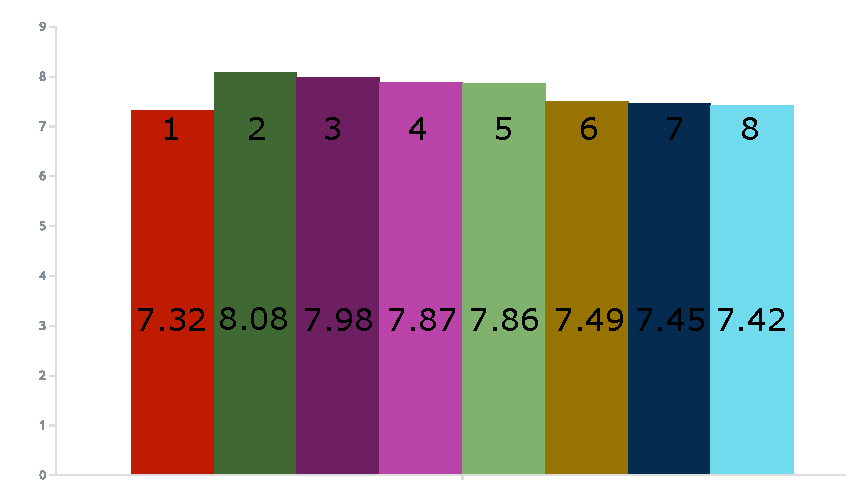
\includegraphics[ width = 11 cm]{img/kriteria.eps}
	\caption{Průměrné skóre kritérií}
	\label{fig:kkk}	
\end{figure}



V tabulce \ref{Korelace_výsledky} jsou výsledky postupné korelace a ne hromadné, protože hromadná korelace je zkreslena vztahy mezi jednotlivými poli, ale nás zajímá pouze vztah mezi polem SCORE\_TOTAL a jednotlivými kritérii.
\begin{table}[h]
	\centering

	\begin{tabular}{|l|c|}
		\hline
		\multicolumn{1}{|c|}{\textbf{Název pole}}    & \textbf{Korelace} \\ \hline
		\textbf{SCORE\_SERVICE\_STAFF}               & 0,8022            \\ \hline
		\textbf{SCORE\_VALUE\_FOR\_MONEY}            & 0,6585            \\ \hline
		\textbf{SCORE\_LOCATION}                     & 0,6337            \\ \hline
		\textbf{SCORE\_ROOM\_COMFORT/STANDARD}       & 0,7187            \\ \hline
		\textbf{SCORE\_FACILITIES}                   & 0,6001            \\ \hline
		\textbf{SCORE\_HOTEL\_CONDITION/CLEANLINESS} & 0,8524            \\ \hline
		\textbf{SCORE\_FREE\_WIFI}                   & 0,5977            \\ \hline
	\end{tabular}
	\caption{Výsledky korelace}
\label{Korelace_výsledky}
\end{table}


Z tabulky \ref{Korelace_výsledky} je jasně patrné, že pole SCORE\_TOTAL nejvíce koreluje s poli SCORE\_SERVICE\_STAFF a SCORE\_HOTEL\_CONDITION/CLEAN- LINESS, což je pro mne překvapující, protože jejich celková průměrná hodnota se liší o 0,7 bodu \todo{opravdu?}. Tato odchylka bude způsobena nejspíše tím, že SCORE\_TOTAL má vyplněno o 23\% více recenzí. Z výsledků lze usoudit, že celkový dojem z hotelu nejvíce ovlivňuje kvalita poskytovaných služeb, ochota personálu, stav a čistota hotelu a také pohodlí pokojů. Lokalita hotelu a přínos návštěvy za vynaložené náklady také ovlivňují celkové skóre, ale podobnou měrou, která je oproti předchozím kritériím výrazně menší. Ze zvolených kritérií naopak nejméně ovlivňuje celkovou známku kvalita poskytované bezplatné WiFi a také úroveň vybavenosti hotelu.

\subsubsection{Jak hodnotí návštěvníci dostupnost veřejné dopravy?}
\label{doprava}
Na tuto otázku nelze  bohužel najít relevantní odpověď. Důvodem jsou sebraná data, ve kterých nejsou vyplněny podrobnosti o dostupnosti veřejné dopravy v okolí hotelu. Jediným zdrojovým polem, ve kterém jsou zmínky o dopravě, popřípadě o veřejné dopravě je pole REVIEW, kde je uložené slovní hodnocení návštěvníka. Bohužel ve většině případů nehodnotili recenzenti možnosti veřejné dopravy. Z celkového počtu 337 302 recenzí, které mají vyplněné pole REVIEW, obsahuje pouze 2873 zmínku o veřejné dopravě, popřípadě o dopravě obecně. Kvůli malému vzorku dat tudíž nelze najít odpověď. která by byla obecně platná. \todo{2. příklady, které nelze zobecnit do 1.}

\chapter{Implementace webových stránek}
\label{chap:WEB}
Další podstatnou částí mé bakalářské práce je implementace webových stránek, které by umožňovaly zobrazit vizualizace, jež během práce vznikly v nástroji Kibana. Samotný nástroj vyžaduje pokročilou znalost s databázemi, a to především kvůli specifickému jazyku Query DSL, který je využíván pro vyhledávání v datech. Pro běžné koncové uživatele může být ovládání problematické a právě to se snažím implementací webových stránek změnit. Kód stránek je uspořádán celkem do tří samostatných souborů a to autocomplete.css, web\_page.html a query.php. První jmenovaný soubor obsahuje pouze úpravu kaskádových stylů a to především pro implementovaný našeptávač. Druhý soubor je hlavní, protože se v něm nalézá HTML kód webových stránek a zároveň obsahuje funkce, které zajišťují chod stránek. Funkce jsou napsány v jazyce JavaScript, protože potřebuji zajistit interaktivitu výsledných stránek. Poslední soubor slouží ke komunikaci s databází Elasticsearch a je využíván jako zdroj dat pro implementovaný našeptávač.

\section{Funkce stránek}
Hlavním přínosem stránek je možnost snadného srovnání dvou různých hotelů. Názvy hotelů se nemusejí zadávat ve speciálním formátu dotazu, ale do patřičných polí stačí pouze zadat název hotelu, popřípadě jej vybrat ze  seznamu našeptávače, který je nasazen na obě vyhledávací pole. Při srovnání si je možné vybrat z několika vizualizací, které lze měnit v rozbalovacím menu. Obsah tohoto menu a tudíž i nabízených vizualizací je možné změnit pouze přímo v souboru web\_page.html, kde lze zároveň i změnit adresu serveru, na kterém běží aplikace Kibana a Elasticsearch. Výhodu taktéž spatřuji v tom, že skrze implementované stránky nijak nelze trvale změnit vlastní vizualizace, které jsou uložené v nástroji Kibana, ale lze je pouze přizpůsobit pro dané srovnání. To je umožněno využitím rozšířeného režimu sdílení, který je nazýván \uv{embeded}. Při srovnání je možné využít taktéž pokročilého nastavení, které je určeno především pro zkušenější uživatele, kteří jsou seznámeni se syntaxí Lucene dotazovacího jazyka. V tomto pokročilém režimu je možné ovlivnit výsledné vizualizace zadáním konkrétních dotazů v patřičném formátu. Stránky umožňují aplikovat pro každý hotel vlastní dotaz, případně je možné zadat pouze jeden dotaz, který se následně aplikuje na oba výsledky a ovlivní zobrazené vizualizace.

\section{Použité technologie}
\subsubsection{Bootstrap}
Bootsrap je populární HTML, CSS a JavaScript Framework určený k vývoji responzivních webových stránek.\cite{Bootsrap} Velkou výhodou je především velké množství HTML prvků, které lze využít a není nutné dále upravovat kaskádové styly, které slouží k zobrazení elementů na webových stránkách. Je možné stáhnout si celou knihovnu s kaskádovými styly na lokální disk a nadále je upravovat, ale já jsem v rámci práce využil hostovaných knihoven, které jsou k dispozici na stránkách \url{https://www.bootstrapcdn.com/}. Výhoda hostovaných knihoven je jejich neustálá inovace, která zajišťuje kompatibilitu zobrazovaných prvků i s novými způsoby zápisu. Zároveň lze ovšem vytvořit separátní lokální CSS soubor, který má před hostovanými knihovnami přednost, čehož jsem využil u prvků, ve kterých je zobrazena výsledná vizualizace z nástroje Kibana. Kromě běžných HTML elementů jako jsou tlačítka, formulářová pole, rozbalovací menu jsem využil speciální druh blokového elementu \uv{div}, který zajišťuje responzivní vzhled obsahu, který tento element obklopuje. Při zobrazování vizualizací jsem narážel na problém s jejich velikostí, která kolidovala s responzivním designem ostatních prvků a na menších zařízeních se tyto prvky překrývaly. Bootsrap poskytuje třídu \uv{embeded-responsive}, která je určená pro vkládání obsahu v prvcích \uv{iframe} a zajišťuje změnu velikosti těchto prvků tak, aby se nepřekrývaly s ostatními prvky na stránce. Je možné si zvolit responzivní design ve formátu 4:3 popřípadě 16:9, kdy jsem zvolil pro mé stránky první možnost, kde lépe vyniknou vizualizace z nástroje Kibana.


Bootstrap jsem zvolil především kvůli zjednodušení práce s designem webových stránek a také kvůli snadné tvorbě responzivních webových stránek, jejichž zobrazení se vždy přizpůsobí danému zařízení.

\subsubsection{HTML5}
HTML5 je nejnovější verze značkovacího jazyka pro tvorbu statických webových stránek. V práci jsem použil elementární prvky tohoto jazyka především ve frameworku Bootstrap a samotné HTML jsem použil jen zřídka.

\subsubsection{JavaScript}
Tento objektově orientovaný skriptovací jazyk zajišťuje implementovaným webovým stránkám jejich interaktivitu. Vlastní skripty jsou umístěny přímo v HTML kódu a jsou celkem dva. Prvním je skript, který obstarává funkci našeptávače pro názvy hotelů a druhý skript naopak zajišťuje komunikaci s nástrojem Kibana, upravuje URl a zobrazuje vizualizace podle uživatelem zadaných parametrů. 


Právě úprava URl je nejpodstatnější, protože skrze něj komunikuji s Kibana a předávám jí název hotelu a případné filtry, které má aplikovat do výsledné vizualizace. Tento způsob komunikace je nevýhodný v tom, že se pokaždé změně musí znovu načíst celá vizualizace, což v závislosti na aktuálním vytížení serveru muže trvat i pár sekund. Vhodnější formou by byla komunikace skrze internals a plugin, který umožňuje komunikovat s prvkem iframe, ve kterém je vizualizace umístěna. Bohužel není toto rozšíření oficiálně podporováno firmou Elastic a je vyvíjeno pouze komunitou a s příchodem nové verze 5.0 je nepoužitelné z důvodu nekompatibility. Komunita se to sice snaží řešit, ale rozšíření je stále ve fázi testování a to již od února 2017. Toto rozšíření se oficiálně jmenuje Kibana iFrame Comunicator a je plně kompatibilní s Kibana ve verzi 4.X.

\subsubsection{jQuery}
V práci jsem také využil javascriptové knihovny jQuery, která umožňuje vývojářům přidat extra funkcionalitu k HTML prvkům a zaměřuje se právě na interakci mezi HTML a JavaScriptem. Tato knihovna je open-source a je dostupná pod licencí MIT\cite{jQuery} , jejíž text vznikl na půdě Massachusetts  Institute of Technology.\cite{MIT_licence} Výhodou je, že funkcionalita nemusí být jednotlivým prvkům přiřazena přímo v HTML kódu, ale lze najít jednotlivé elementy skrze jejich unikátní identifikátory a posléze jim přiřadit funkcionalitu až ve skriptu. Této možnosti jsem využil, a na základě akcí typu kliknutí myši, stisk klávesy, jsem přiřadil jednotlivým tlačítkům a formulářovým prvkům funkce v JavaScriptu.

\paragraph{Autocomplete}
\mbox{}\\
Pro zjednodušení zadávání názvů hotelů jsem se rozhodl implementovat do webových stránek našeptávač. K tomu jsem použil rozšíření Autocomplete, které je součástí jQuery uživatelského rozhraní. Toto rozšíření poskytuje koncovým uživatelům možnost snadno si vybrat a zadat název konkrétního hotelu, protože jim dává k dispozici jejich seznam, který se aktualizuje podle uživatelského vstupu. Implementace tohoto rozšíření je velmi jednoduchá, protože jej stačí jen napojit na prvek, který obstarává uživatelský vstup. Problémem mohou být pouze ostatní elementy na stránce, které mohou být zobrazeným seznamem překryty. Způsobeno je to tím, že zobrazuji všechny odpovídající názvy hotelů a rozbalovací menu se automaticky přizpůsobí počtu záznamů. Tento problém je vyřešen souborem autocomplete.css, ve kterém definuji pevnou výšku rozbalovacího menu.


Našeptávač potřebuje také zdrojová data, ve kterých hledá relevantní výsledky, které obsahují řetězec zadaný koncovým uživatelem. Zdrojová data musí být ve formátu JSONP, který je stejný jako formát JSON, ale je navíc uzavřen v závorce. Tento formát slouží k asynchronní komunikaci klientské aplikace se serverem prostřednictvím technologie AJAX, která je popsána níže. Rozšíření bere v mém případě data z prostého javascriptového pole s názvy hotelů. Toto pole se automaticky aktualizuje pomocí PHP souboru, když uživatel změní vstupní řetězec. Našeptávač by také mělo být možné přímo napojit na PHP soubor pomocí technologie AJAX, ale bohužel i přes správný formát JSONP tento postup nefungoval a proto využívám okliku v podobě javascriptového pole.


Stejně jako u Bootstrap jsem namísto lokálních souborů využil hostované knihovny a to konkrétně od Google, které jsou k dispozici na stránce\\ \url{https://developers.google.com/speed/libraries/}.

\subsubsection{AJAX}
Další použitou technologií je AJAX, která umožňuje asynchronní komunikaci se serverem a pro změnu obsahu stránek tak není nutné jejich kompletní znovunačtení. Tato technologie také zajišťuje interaktivitu webových stránek. Konkrétně jsem využil příkaz \$.ajax, který je dostupný v knihovně jQuery. Tento příkaz slouží k zasílání HTTP požadavku serveru a v případě úspěchu je možné s výsledkem nadále pracovat. Hlavním parametrem je URl adresa serveru, se kterým chceme navázat komunikaci. V mém případě se jedná o soubor query.php, kterému předávám řetězec z uživatelského vstupu. URl tedy bude adresa serveru a následované umístěním souboru query.php. Po úspěšném požadavku zpracuji odpověď serveru a uložím hodnoty reprezentující názvy hotelů do pole, které používám jako zdrojové pole pro našeptávač.


Problémem při použití asynchronní komunikace je CORS, neboli Cross-origin resource sharing. Moderní webové prohlížeče očekávají v odpovědi serveru hlavičku s informací o CORS, podle které definují omezení o sdílení zdrojů. Na straně serveru tak může být nastavena podpora sdílení pouze pro určité URl adresy. V mé práci používám jako server, na kterém běží PHP soubor, aplikaci WampServer a pro úspěšnou komunikaci je nutné nejprve povolit v nastavení Apache \uv{headers\_module} a následně přidat do souboru \uv{http.conf} přidat řádek: \uv{Header add Access-Control-Allow-Origin „*“}.

\subsubsection{PHP}
PHP je serverový skriptovací jazyk, který umožňuje tvorbu dynamických a interaktivních webových stránek.\cite{PHP} V případě nově vzniklých webových stránek jsem tento jazyk využil pro dotazování se do databáze Elasticsearch, ze které následně získávám data pro našeptávač. PHP jsem zvolil z důvodu snadné implementace komunikace se serverem s běžící databází Elasticseach pomocí příkazů curl. PHP nativně podporuje knihovnu libcurl, která umožňuje připojení a komunikaci se servery.\cite{PHP_libcurl} Důležité je, že lze skrze libcurl zaslat HTTP dotaz typu POST, pomocí kterého je umožněna komunikace s databází Elasticsearch.


Soubor query.php získá z javascriptového skriptu vstupní parametr, který následně odešle databázi Elasticsearch vhodným dotazem, jehož forma je popsána v sekci Zdrojová data pro našeptávač. V souboru používám hlavně funkce jazyka PHP pro  práci s řetězci, protože hlavním úkolem tohoto skriptu je získání dat pro našeptávač ve vhodném formátu.

\section{Zdrojová data pro našeptávač}
Největší problém při implementaci stránek byla bezesporu tvorba našeptávače, který by koncovým uživatelům napomáhal s výběrem hotelů. Důležitou vlastností pro našeptávač je rychlost, protože uživatelé potřebují dynamicky se měnící obsah rozbalovacího menu, ze kterého si mají vybrat hotel. Jak již bylo zmíněno výše, použil jsem Autocomplete, což je součást knihovny jQuery UI, který obstarává zobrazení relevantních návrhů, dále pak technologii AJAX pro zasílání požadavků PHP serveru, jenž komunikuje přímo s databází Elasticsearch a získává názvy hotelů a předává je ve vhodném formátu. Důležitá je také rychlost, jakou databáze prohledá záznamy a vrátí ty vhodné.

\subsubsection{Completion Suggester}
V databázi Elasticsearch lze vytvořit speciální pole datového typu \uv{comple\-tion}, které je přímo určené pro navázání na našeptávač. V dokumentaci se píše, že poskytuje okamžitou odezvu na zadaný dotaz, jelikož je toto pole díky speciálnímu datovému typu optimalizováno na rychlé vyhledávání.\cite{Completion_suggester}


Datová struktura poskytuje rychlé prohledávání databáze za cenu vysokého využití paměti, jelikož ukládá data do hlavní paměti serveru, na kterém běží. Jedná se tak o přístup in-memory. V této struktuře jsou uložena klíčová slova (v našem případě názvy hotelů) a je z nich vytvořen graf. Pokud by struktura obsahovala klíčová slova \uv{Villa}, \uv{Royal} a \uv{Royalton}, byl by výsledkem graf \ref{fig:Completer}.

\begin{figure}[h]
	\centering
	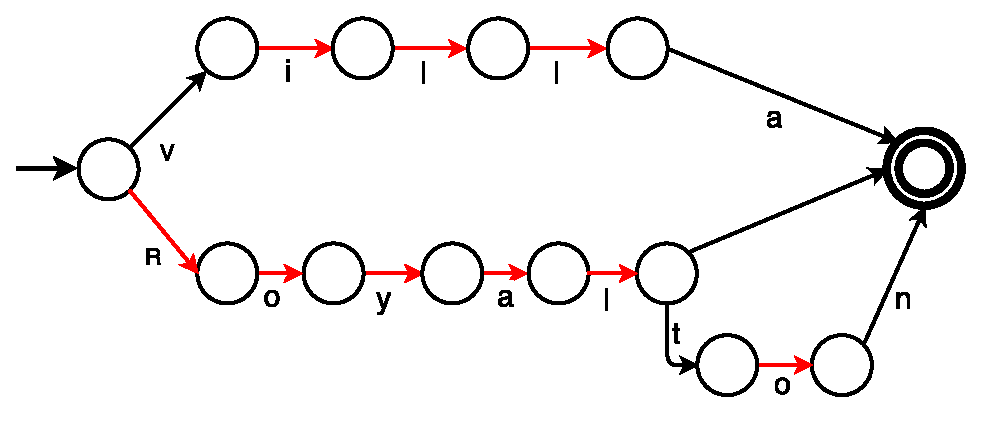
\includegraphics[ width =8cm]{img/completer.eps}
	\caption{Graf Completion Suggester}
	\label{fig:Completer}	
\end{figure}


Jakmile by tedy uživatel zadal písmeno \uv{v}, vrátila by databáze \uv{Villa}.


Rychlost vyhledávání se samozřejmě postupem času zvyšuje, protože nejnáročnější je na procesu našeptávání tvorba grafu, který je uložen v paměti, ale zároveň při novém dotazu pouze doplní a nemusí se tudíž tvořit nový graf.


Formát dotazu je podobný jako u jiných dotazů pro Elasticsearch. V mém případě přidávám  do dotazu parametr \uv{\_source:HOTEL\_NAME}, kterým specifikuji, že žádám pouze od navrácení hodnot pole HOTEL\_NAME.
\begin{lstlisting}[title={Zápis completion dotazu}]
		POST index/_search?pretty{
		 "suggest":{
	  	  "hotel-suggest":{
		   "prefix": vstup,
		   "completion": {
		    "field":"suggest_field",
		    "size":2500
		}}}}
\end{lstlisting}

\subsubsection{Způsob získání dat}
Jakmile uživatel zadá do vyhledávacího pole nějaký vstup, je tento vstup pomocí skriptu přeposlán do souboru query.php, který následovně pošle dotaz v patřičném formátu, který je uveden výše do Elasticsearch. Zdrojová pole pro našeptávač v Elastisearch jsou pole \uv{HOTEL\_NAME\_SUGGEST} a \uv{HOTEL\_NAME\_SUGGEST\_TOKENS}. Druhé pole je vhodné pro vyhledávání jednoslovných řetězců a první pole je vhodné pro doplňování přesného názvu hotelu.


Odpověď serveru s běžící databází Elasticsearch je následně pomocí dvou cyklů zpracována do pole, které ovšem obsahuje duplicitní údaje, jelikož odpověď může obsahovat až 2500 záznamů. Z tohoto důvodu je pole následně seřazeno pomocí funkce \uv{sort} a následně funkcí \uv{array\_unique} získám PHP pole obsahující unikátní názvy hotelů, jež jsou následně převedeny do formátu JSONP. Právě pole s názvy hotelů ve formátu JSONP je následně vráceno do skriptu v souboru web.html a slouží jako zdrojové pole pro našeptávač realizovaný pomocí Autocomplete rozšíření.

\chapter{Závěr}
\label{závěr}
V rámci práce jsem provedl průzkum trhu s BI nástroji a detailně jsem prostudoval pět nástrojů, které se jevily jako vhodné pro zpracování dat z ubytovacích portálů. Informace o jednotlivých  produktech jsem získával z oficiálních dokumentací, uživatelských recenzí a ze stránek, které se problematice zpracování a vizualizace dat zabývají. Funkce jednotlivých nástrojů jsem vypozoroval z demonstračních videí, ale vhodnější by bylo funkcionalitu ověřit přímo na konkrétních datech. To ovšem nebylo možné, protože jednotlivé nástroje nebyly přímo kompatibilní s databází Elasticsearch. Výsledkem průzkumu je zvolení dle mého názoru nejvhodnějšího nástroje k vizualizaci dostupných dat, kterým je nástroj Kibana. Více o zkoumaných nástrojích se lze dohledat v kapitole \ref{Nástroje_1}.


Přehled základních funkcí a jejich popis je dostupný v kapitole \ref{Funkce_nástroje}. Jelikož je ovládání většiny funkcí intuitivní, zaměřil jsem se hlavně na vysvětlení Query DSL, principu vyhledávání a na rozšíření Graph, které jsem následně využil při vizualizaci vybraných otázek.


Hlavním přínosem práce jsou odpovědi na vybrané otázky, které jsem obdržel společně se zadáním. Celkem jsem odpověděl na deset otázek a odpovědi jsem podpořil vizualizacemi, které byly vytvořeny v nástroji Kibana, případně v aplikaci Microsoft Excel. K odpovědím, které byly složité na vypracování, jsem kromě vlastní odpovědi a vizualizace také připojil část, popisující jak jsem při jejich tvorbě postupoval, aby byly výsledky reprodukovatelné. 


Další přínosem je implementace interaktivního webu, jehož hlavní funkcí je možnost srovnat dva vybrané hotely. Ke srovnání slouží různé vizualizace, mezi nimiž si může uživatel webu vybrat. Vizualizace může ovšem přidat pouze administrátor  webu a to přímo do HTML kódu. Zde vidím možnost pro budoucí zlepšení, kdy by se zobrazovaly všechny vizualizace, které jsou uložené v nástroji Kibana. Výhodou webových stránek je možnost ovlivnění zobrazené vizualizace zadáním názvu hotelu do vstupního pole, bez nutnosti znalosti  dotazovacího jazyka. Zároveň je na vstupní pole napojen našeptávač, který tento výběr usnadňuje. Pro  zkušenější uživatele je možnost dalšího ovlivnění vizualizací zadáním dotazu, který respektuje syntaxi dotazovacího jazyka Lucene. Do budoucna by se na webových stránkách dala zcela jistě vylepšit grafická podoba, která je nyní prostá. Dalším možným vylepšením by mohlo přidání pole pro zadávání dotazů, které by již nemusely respektovat formát Query DSL a umožnit tak běžným uživatelům více filtrovat data.



\chapter{Slovník pojmů}
\label{Slovník}



\hspace{0,5cm} \textbf{BI:} \uv{Business intelligence, nebo také BI, je rámcový termín, označující paletu softwarových aplikací využívaných k analýze raw dat organizace.} \cite{BI}

\textbf{Big Data:} \uv{je termín aplikovatelný na soubory dat, jejichž velikost je mimo schopnosti zachycovat, spravovat a zpracovávat data běžně používanými softwarovými nástroji v rozumném čase.} \cite{BigData}

\textbf{CRM} neboli Customer Relationship Management je zkratka pro podpůrné informační systémy, které jsou určené pro řízení vztahů se zákazníky.

\textbf{CSV} neboli Comma-separated values je souborový formát určený pro výměnu tabulkových dat. Soubor se skládá z řádků, na kterých jsou uložené položky, které jsou od sebe odděleny oddělovači (například čárka, středník, tabulátor atd.).

\textbf{JSON} \uv{neboli JavaScript Object Notation je formát souborů určený k výměně dat.} Je snadno čitelný i zapisovatelný člověkem a zároveň lze soubory ve formátu JSON snadno generovat i zpracovávat strojově.\cite{JSON}

\textbf{NoSQL}\uv{Jedná se o novou generaci databázových systému pro správu velkého množství dat, které jsou převážně ne-relační, distribuované, škálovatelné a podporují replikaci. Často jsou to databáze bez datového schématu, s jednoduchým rozhraním pro práci s daty a open source přístupem}.\cite{NoSQL}

\textbf{Materializovaný pohled:} jsou to databázové objekty obsahující výsledek dotazu. Přístup k výsledku je rychlejší než u normálních query dotazů, ale nesmí se měnit vstupní data pro materializovaný pohled, protože se neaktualizuje automaticky při změně databáze.

\textbf{PDF} \uv{PDF neboli Portable Document Format je formát používaný k prezentaci a spolehlivé výměně dokumentů, který je nezávislý na softwaru, hardwaru i operačnímu systému.} \citealp{PDF}

\textbf{SOAP:} Simple Object Access Protocol je protokol zajišťující přenos zpráv založených na XML přes síť, především pak pomocí protokolu HTTP.

\textbf{XML:} neboli Extensible Markup Language je obecný značkovací jazyk určen pro uchování a přenos dat. Je čitelný jak pro lidi tak i pro stroje.

\bibliographystyle{csplainnatkiv}
{\raggedright\small
\bibliography{literatura}
}

\end{document}
